%%
%% Copyright 2007, 2008, 2009 Elsevier Ltd
%%
%% This file is part of the 'Elsarticle Bundle'.
%% ---------------------------------------------
%%
%% It may be distributed under the conditions of the LaTeX Project Public
%% License, either version 1.2 of this license or (at your option) any
%% later version.  The latest version of this license is in
%%    http://www.latex-project.org/lppl.txt
%% and version 1.2 or later is part of all distributions of LaTeX
%% version 1999/12/01 or later.
%%
%% The list of all files belonging to the 'Elsarticle Bundle' is
%% given in the file `manifest.txt'.
%%

%% Template article for Elsevier's document class `elsarticle'
%% with numbered style bibliographic references
%% SP 2008/03/01
%%
%%
%%
%% $Id: elsarticle-template-num.tex 4 2009-10-24 08:22:58Z rishi $
%%
%%
\documentclass[preprint,12pt]{elsarticle}
\biboptions{sort&compress}

%% Use the option review to obtain double line spacing
%% \documentclass[preprint,review,12pt]{elsarticle}

%% Use the options 1p,twocolumn; 3p; 3p,twocolumn; 5p; or 5p,twocolumn
%% for a journal layout:
%% \documentclass[final,1p,times]{elsarticle}
%% \documentclass[final,1p,times,twocolumn]{elsarticle}
%% \documentclass[final,3p,times]{elsarticle}
%% \documentclass[final,3p,times,twocolumn]{elsarticle}
%% \documentclass[final,5p,times]{elsarticle}
%% \documentclass[final,5p,times,twocolumn]{elsarticle}


% Users' option
\usepackage{amssymb}
\usepackage{amsmath}
\usepackage{graphicx}
\usepackage{epstopdf}
\usepackage{color}
\usepackage{array}
\topmargin=0.001in
\usepackage{multirow}
\usepackage{booktabs}
\usepackage{subfig}
\newif\ifdraft
\drafttrue

\renewcommand{\multirowsetup}{\centering}
\renewcommand{\arraystretch}{1.2}
\def\nyc{\centering}

\ifdraft
\newcommand{\fixme}[1]{ { \bf{ ***FIXME: #1 }} }
\newcommand{\jhanote}[1]{ {\textcolor{red} { ***Jha: #1 }}}
\newcommand{\Nkimnote}[1]{ {\textcolor{blue} { ***NKim: #1 }}}
\newcommand{\skonote}[1]{ {\textcolor{green} { ***Jeff: #1 }}}
\newcommand{\cand}[1]{ {\bf\textcolor{blue} { ***Or: #1 }}} 
\else
\newcommand{\jhanote}[1]{}
\newcommand{\Nkimnote}[1]{}
\newcommand{\fixme}[1]{}
\newcommand{\skonote}[1]{}
\newcommand{\cand}[1]{}
\fi

\newcommand{\up}{\vspace*{-1em}}
\newcommand{\upp}{\vspace*{-0.5em}}
\newcommand{\ts}{$T_{s}$}

\newcommand{\superscript}[1]{\ensuremath{^{\textrm{#1}}}}
\newcommand{\subscript}[1]{\ensuremath{_{\textrm{#1}}}}

\newcommand{\lb}[0]{\subscript{LB} }
% End of users' option



\journal{Journal of Computational Science}

\begin{document}

\begin{frontmatter}
%% Title, authors and addresses

%% use the tnoteref command within \title for footnotes;
%% use the tnotetext command for the associated footnote;
%% use the fnref command within \author or \address for footnotes;
%% use the fntext command for the associated footnote;
%% use the corref command within \author for corresponding author footnotes;
%% use the cortext command for the associated footnote;
%% use the ead command for the email address,
%% and the form \ead[url] for the home page:
%%
%% \title{Title\tnoteref{label1}}
%% \tnotetext[label1]{}
%% \author{Name\corref{cor1}\fnref{label2}}
%% \ead{email address}
%% \ead[url]{home page}
%% \fntext[label2]{}
%% \cortext[cor1]{}
%% \address{Address\fnref{label3}}
%% \fntext[label3]{}


\title{Accurate and Efficient Multi-scale Flow Simulation using a Hybrid CFD-MD Approach}
\author[add0,add1]{Soon-Heum Ko}
\ead{sko@nsc.liu.se}
\author[add1]{Nayong Kim}
\ead{nykim@cct.lsu.edu}
\author[add3]{Dimitris Nikitopoulos}
\ead{meniki@me.lsu.edu}
\author[add3]{Dorel Moldovan}
\ead{moldovan@me.lsu.edu}
\author[add1,add2]{Shantenu Jha\corref{Corr}}
\ead{sjha@cct.lsu.edu}
\address[add1]{Center for Computation \& Technology, Louisiana State University, Baton Rouge, LA 70803, USA}
\address[add0]{National Supercomputing Centre, Link\"{o}ping University, Link\"{o}ping, SE-581 83, Sweden}
\address[add2]{Department of Computer Science, Louisiana State University, Baton Rouge, LA 70803, USA}
\address[add3]{Department of Mechanical Engineering, Louisiana State University, Baton Rouge, LA 70803, USA}
\cortext[Corr]{Corresponding author, (Tel)+1-225-578-XXXX; (FAX)+1-225-578-XXXX}

\begin{abstract}
Reduction of statistical error in molecular dynamic samples and time-accurate temporal coupling scheme are important numerical issues associated with hybrid computational fluid dynamics (CFD) - molecular dynamics (MD) simulation methodologies. Also, effective scheduling of distinct-yet-coupled codes on computing resources is necessary for the efficiency of this computationally-intensive simulation. In this paper, we introduce our developments and implementations to resolve above-stated issues. We build our hybrid simulation package by deploying a constrained Lagrangian dynamics scheme with its interface on distinct CFD and MD codes. Statistical error in molecular dynamic sample is minimized by the delicate determination of coupling parameters along with the adoption of replica sampling approach. We introduce a temporal coupling scheme based on a 'prediction-correction' way together with interpolation in time, which provides a more time-accurate hybrid constraint/boundary condition. With respect to computational performance, we employ a Pilot-job abstraction and implement the load-balancing function to provide co-scheduling and load-balancing between logically distributed tasks on the batch queue. We apply our hybrid simulation framework to solving two classical flow problems of the impulsively started Couette flow and an oscillating boundary Stokes flow. Results verify that the multiple replica sampling contribute much on suppressing the sampling noise. Also, the accuracy of unsteady flow solution is increased by applying a 'prediction-correction' temporal coupling scheme. Finally, a Pilot-job abstraction contributes to saving computational cost by eliminating idle waiting of first-started task and efficiently distributing allocated resources to coupled tasks.
\end{abstract}

\begin{keyword}
Hybrid computational fluid dynamics - molecular dynamics approach 
\sep Constrained Lagrangian dynamics 
\sep Temporal coupling scheme 
\sep Simple API for Grid Applications (SAGA)
\sep Pilot-job abstraction
\end{keyword}

\end{frontmatter}



%% main text
\section{Introduction and Motivation}
\label{sec:intro}

A hybrid continuum dynamics - particle dynamics approach is an approach 
capable of describing accurately a flow at both macroscopic and molecular scales. 
In this approach the system is divided into two domains. 
A continuum formulation is used appropriately for one domain and 
a particle formulation (e.g. molecular dynamics) is applied to the other.
Naturally the particle domain is more appropriate for material interfaces 
(e.g. fluid/solid or fluid/fluid) where molecular effects are more likely to be important. 
On the other hand, the continuum approach provides a better computational efficiency than
particle dynamics with acceptable accuracy in solving the bulk flow field.
In the hybrid approach the two domains are coupled through an overlap region/interface 
in which both formulations are valid. The overlap domain enables the exchange of 
conservative flow properties between the continuum and particle ones so that 
the respective solutions are mutually consistent. 
The information from the continuum domain is passed to the particle domain 
by imposing additional numerical modeling to preserve higher degree-of-freedom 
on the particle motion, while the particle domain provides boundary conditions 
to the continuum domain obtained through time and spatial averaging of the relevant variable.

Despite the recent developments reported in the literature, most of which tested 
against small idealized pure atomistic flow simulations for comparison, 
there are still methodological and implementation issues that need refinement, 
testing and validation. In this section, we will give a brief account of the numerical and 
computational issues associated with some of the previous hybrid CFD-MD implementations 
and outline our approach to address them effectively.


\subsection{Previous Hybrid CFD-MD Implementations}
\label{sec:intro_formerworks}

Hybrid CFD-MD simulations have utilized constrained Lagrangian dynamics~\cite{Thompson,Nie,Nie_cavity,Cui,Wang,Yen,Liu}, the Schwarz method~\cite{Hadjicon1,Hadjicon2,Hadjicon3,Werder,Kotsalis}, or a direct flux exchange~\cite{Flekkoy,Wagner,Delgado1,USHER,Time_Mechanism,Giupponi} method, depending on the methodology used to impose the solution matching in the overlap region/interface and the nature of the variables that exchange information in this region. 
O'Connell and Thompson~\cite{Thompson} 
were among the first to implement a hybrid CFD-MD simulation approach by introducing the overlap region that allows matching of the solutions from the two domains to relax smoothly before they are coupled together. Namely, they employed a relaxation method according to which the average MD velocity in an overlap region is forced to follow the continuum solution in the same region. In their implementation they use constrained Lagrangian dynamics according to which the particles are accelerated/decelerated in the overlap region so that on average they follow the continuum velocity. The drawback of their implementation is the arbitrariness of the relaxation rate and the lack of particle exchange (particle flux) between the two domains. 
This approach is refined by Nie {\it{et al.}}~\cite{Nie} 
who imposed the spatial coupling between continuum equations and molecular dynamics through constrained dynamics implemented in the overlap region.
The methodology has been applied to a variety of flow problems such as the impulsively started Couette flow~\cite{Thompson}, channel flow with rough walls~\cite{Nie}, cavity flow~\cite{Nie_cavity}, Poiseuille flow~\cite{Yen} and the oscillating boundary problem~\cite{Wang,Liu}. The use of direct constrained dynamics equation makes this approach easy to implement and computationally efficient. However, the absence of energy exchange modeling limits the applications to isothermal systems~\cite{Flekkoy}.

To alleviate some of these shortcomings, Hadjiconstantinou {\it{et al.}}~\cite{Hadjicon1,Hadjicon2,Hadjicon3} 
have introduced a new hybrid simulation methodology based on the Schwarz method. In this approach, the continuum solution is used to generate the solution in the particle domain in which the particle velocities are drawn from a Maxwellian distribution such that the mean velocity and the corresponding standard deviation are determined by the continuum solution and temperature~\cite{Hadjicon2}. This approach later was expanded to non-periodic boundary condition problems by Werder {\it{et al.}}~\cite{Werder}, who also expanded and refined the previous boundary force models~\cite{Thompson,Flekkoy,Delgado1,Nie} so as to minimize local disturbance. 
An alternating Schwarz approach has been applied to the moving contact line problem~\cite{Hadjicon2}, Poiseuille flow~\cite{Hadjicon3}, flow around the cylinder~\cite{Werder}, and Couette flow of water~\cite{Kotsalis}. The characteristics of decoupled physical time-scales between two domains makes this approach appealing when solving the flow field in problems in which hydrodynamic characteristic time scale is much larger than molecular dynamic time scale, i.e., micrometer system size~\cite{Hadjicon2}. 


In order to be able to simulate isothermal compressible flow, Flekk$\phi$y {\it{et al.}}~\cite{Flekkoy} introduced a new hybrid method based on continuity of mass and momentum fluxes across the MD-continuum interface, which later included energy transfer~\cite{Wagner,Delgado1}. Further developments were implemented by Delgado-Buscalioni and Coveney~\cite{USHER} by introducing a particle insertion algorithm which satisfies the continuity of the mass flux along the interface while preserving the mean potential energy of the system. This approach has been applied to the study of Couette and Poiseuille flow~\cite{Flekkoy}, transversal wave~\cite{Delgado1}, and oscillating boundary problem~\cite{Time_Mechanism}. According to Flekk$\phi$y {\it{et al.}}~\cite{Flekkoy}, flux exchange directly implies adherence to the relevant conservation laws without the use of constitutive relations and equations of state (to maintain the conservation laws). However, it is pointed out that the sampling time to measure fluxes within acceptable statistical error is orders of magnitude larger than the time to measure densities~\cite{Hadjicon3}.



\subsection{Numerical and Computational Issues Associated with Hybrid CFD-MD Methodologies}
\label{sec:intro_issues}

Despite the recent developments and obvious advantages of a hybrid approach for flowing systems with scales straddling molecular to macroscopic (continuum) magnitudes over pure CFD or MD, a number of numerical and computational difficulties prevent this technique from being widely used.
One of the difficulties is the lack of a clear methodology for defining an optimized set of parameters related to the coupling of the continuum and molecular domains. 
In general the flow solution obtained by a direct hybrid approach suffers from the existence of significant noise in the spatially averaged particle velocity mainly due to the inherent statistical fluctuations in the molecular description. Therefore, coupling parameters such as the size of the overlap domain and its position, the width of various layers and bins in the overlap region, and the sampling conditions, should be appropriately determined a priori in order to achieve more accurate numerical solutions.
Many of these coupling parameters are problem dependent and this complicates the problem even further. 
Given the stochastic nature of the noise characterized by the mean velocities in the molecular domain of the coupling region, the characteristics of fluid and solid elements, as well as the geometric characteristics of material (e.g. fluid/solid) interfaces, it is difficult to develop a mathematical model capable of predicting the optimum coupling parameters. 
There have been some attempts to mitigate the inaccuracies associated with inherent statistical fluctuations by introduction of certain numerical damping terms in the equations of motion of the atoms in the overlap region~\cite{Thompson,Cui} or by defining a specific dynamic parameter to controlling the coupling intensity~\cite{Wang}, but all of these eventually lead to some violation of energy and momentum conservation. 

Important issues remain to be addressed in the hybrid implementations for studying flow physics at moderate or low velocity conditions.  So far, most of the reported studies have been confined to relatively high-speed flow conditions, of the order of 100 m/s, in nanoscale systems; flow conditions chosen mainly to obtain a high speed shear rate in the overlapping region and, more importantly, to reduce the relative stochastic thermal noise associated with the velocity flow field~\cite{Yen}. According to the mathematical models~\cite{Hadjicon3,Time_Mechanism} the noise level characterizing the average velocity in the coupling region in a hybrid CFD-MD implementation is proportional to ${{1} / {{u}_{\infty}}^2}$, where the ${u_{\infty}}$ is the far field stream velocity, and to ${{1} / {N_0}}$, where ${N_0}$ denotes the number of particles contained in the sampling layer. Therefore, by reducing the free stream velocity by, say, 10 times, in order the maintain the same noise level (same statistical error)  would require the increase of the number of particles in the averaging bins by 100 times, assuming that the sampling duration is maintained constant. In general the increase of the sampling duration beyond the limits imposed by the physical time-scales of a given unsteady flow problem is to be avoided because it leads to unphysical effects.

The accuracy of temporal coupling schemes is of great importance when solving unsteady problems. In general the temporal coupling scheme encompasses the timing of data exchange between the CFD and MD solvers, so as to synchronize both solutions at the same physical time instant. In this one has to keep in mind that the interpretation of the term "instantaneous" regarding values of variables differs between the continuum and molecular formulations. The time-coupling models are inherently affected by time-lagging. This is more pronounced when backward-averaged molecular dynamic properties are in general communicated as instantaneous properties to the continuum domain. To address this shortcoming, Liu {\it{et al.}}~\cite{Liu} proposed a multi-timescale algorithm by considering quasi-steadiness and Wang and He~\cite{Wang} proposed passing the extrapolated continuum solution to the MD solver. Despite their success there are, however, serious limitations with these approaches as a multi-timescale algorithm is only valid if the characteristic time of the unsteady phenomenon is substantially longer than the integration (averaging) time of the MD solutions. This is also a prerequisite for the particle (MD) solution to be able to equilibrate subject to the constraint passed on from the continuum solution from one continuum time instant to another. The approach by Wang and He may therefore be a good compromise that may mitigate some of the time-lagging effects.

In addition to the above mentioned issues, there are computational challenges related to the integration of multiple application domains into a single problem set. Due to their very different computational kernels (e.g. one mesh-based, the other an unstructured particle-based), it is difficult to incorporate distinct CFD and MD codes under the umbrella of a single tightly-coupled application (i.e. unifying two application codes to share a single MPI communicator). One possible alternative can be to implement a coupling interface into one of the individual codes and design it such that this assumes control of the two separate codes as a virtually unified simulation package. This heterogeneous implementation raises additional computational challenges. For example, in the parallel execution of such a simulation package, on conventional production systems with batch queues, it cannot be guaranteed that two separate jobs will execute concurrently. Considering the computational characteristics of the current application, where the CFD and MD codes conduct frequent data exchange, the first job that completes a task will inevitably experience the idle waiting for its counterpart to finish its sequenced task without the explicit support for co-scheduling. Another important challenge is the need for efficient load-balancing which takes into account the individual application's performance. Even if the two simulations could run concurrently, without explicit load-management/balancing support, there is likely to be inefficient utilization of computing resources due to load imbalance. As the performance of each simulation component changes with computing resource and problem size, re-adjustment of allocated resources to each task according to their performance is required during the hybrid simulation.



\subsection{Objectives and Outline of the Paper}
\label{sec:intro_contents}

The focus of this paper is to investigate numerical issues associated with the implementation of a typical hybrid CFD-MD methodology applied to investigate the flow in a nano/micro-fluidic system as well as with designing and developing of an efficient runtime framework for coupled multi-scale simulations. We present our implementation of a 'generic' hybrid CFD-MD interface which can be easily put together from various 'off the shelf' incompressible CFD and MD packages, as well as our model of a 'portable' framework that can be ported easily on most present day computer architectures. 

We present the development of our hybrid simulation framework, based on constrained Lagrangian dynamics, and apply it to two prototype classical flow problems: the impulsively started Couette flow and an oscillating boundary Stokes flow.
From the pure MD solution on zero-velocity flow field, we elaborate on our strategy for determining the optimized set of coupling parameters that minimize the level of the statistical noise characterizing the flow field obtained by the hybrid solver. 
In addition we extend our investigation into the moderate-speed flow regime (flow velocities of the order of 10 m/s), which is challenging and novel. The inherent large fluctuations of the solution in the overlap region associated with relatively low flow speed are reduced by a multiple replica averaging methodology. For the oscillating boundary Stokes flow simulation, we demonstrate a novel temporal coupling scheme, called 'prediction-correction approach' which provides improved accuracy by eliminating the overshoot/undershoot phenomena and diminishes the time-lagging pattern.

In terms of computational science, our study introduces a novel approach to coupled multi-physics simulations by utilizing the virtually unified simulation package, called "Pilot-Job". We argue that using the Pilot-Job approach has distinct advantages, such as: (i) elimination of the need for a co-scheduler while preserving performance, and (ii) enables dynamic resource allocation, which in turn is important for load-balancing across coupled simulations. 

The paper is organized as follows. In Section~\ref{sec:numerical} we give a brief description of the fundamental equations describing the CFD and MD formulations as well as details of the hybrid CFD-MD coupling scheme and its implementation. Technical details related to the implementation of an efficient CFD-MD simulation framework are presented in Section~\ref{sec:computational}. In Section~\ref{sec:accuracy}, we present the solutions to the two prototype problems (impulsively started Couette flow and oscillating boundary Stokes problem) obtained with our hybrid methodology. The performance and the optimization issues related to the solutions of the two test problems are described in Section~\ref{sec:performance}. Conclusion and future works are presented in Section~\ref{sec:conclusion}.



% -------------------------------------------------------------------------
\section{Fundamentals of the Hybrid Coupled CFD-MD Simulation Toolkit}
\label{sec:numerical}

The accuracy of a hybrid CFD-MD solution is governed by the underlying numerical schemes of the individual continuum and particle solvers as well as the coupling scheme. This section details and explains the features of baseline solvers and the structure of the hybrid coupling interface. Additional numerical treatments to improve the accuracy of hybrid CFD-MD simulations in various types of fluid systems are also addressed.


\subsection{Overview of the Continuum-Molecular Coupled Approach}
\label{sec:numerical_hybridoverview}

The hybrid CFD-MD approach stands on the proposition that (a) the molecular dynamic simulation produces a more physically accurate solution in its domain than the continuum model would, (b) a faster and more efficient CFD solver provides a physically accurate solution in the continuum domain, which would be prohibitive if a particle representation were to be used, and (c) the two solutions can be reconciled by the mutual exchange of information, the continuum solution providing the constraint to the particle solution while the latter providing a boundary condition to the former. So, the region within which molecular-level physics are important (e.g. a material interface) is treated and resolved by a molecular dynamic simulation, while the region within which the continuum-level physics adequately represent the transport processes on a macroscopic scale is treated and resolved by the continuum CFD. The continuum and particle (molecular) domains overlap, in this approach, so as to exchange information for the coupling. Obviously, the overlap domain must be one where both treatments/formulations are valid.

A detailed structure of the various domains associated with the hybrid CFD/MD methodology is described in Fig. 1. CFD solves the continuum equations in the ''pure CFD region'' while MD resolves the microscopic (particle) flow in the ''pure MD region'' The latter is a solid stationary wall for the two test problems examined herein. The hybrid (overlap) region is placed sufficiently far from the solid wall to prevent direct constraint of the molecular-level physics in the proximity of the solid-fluid interface. 


\begin{figure}
\centering
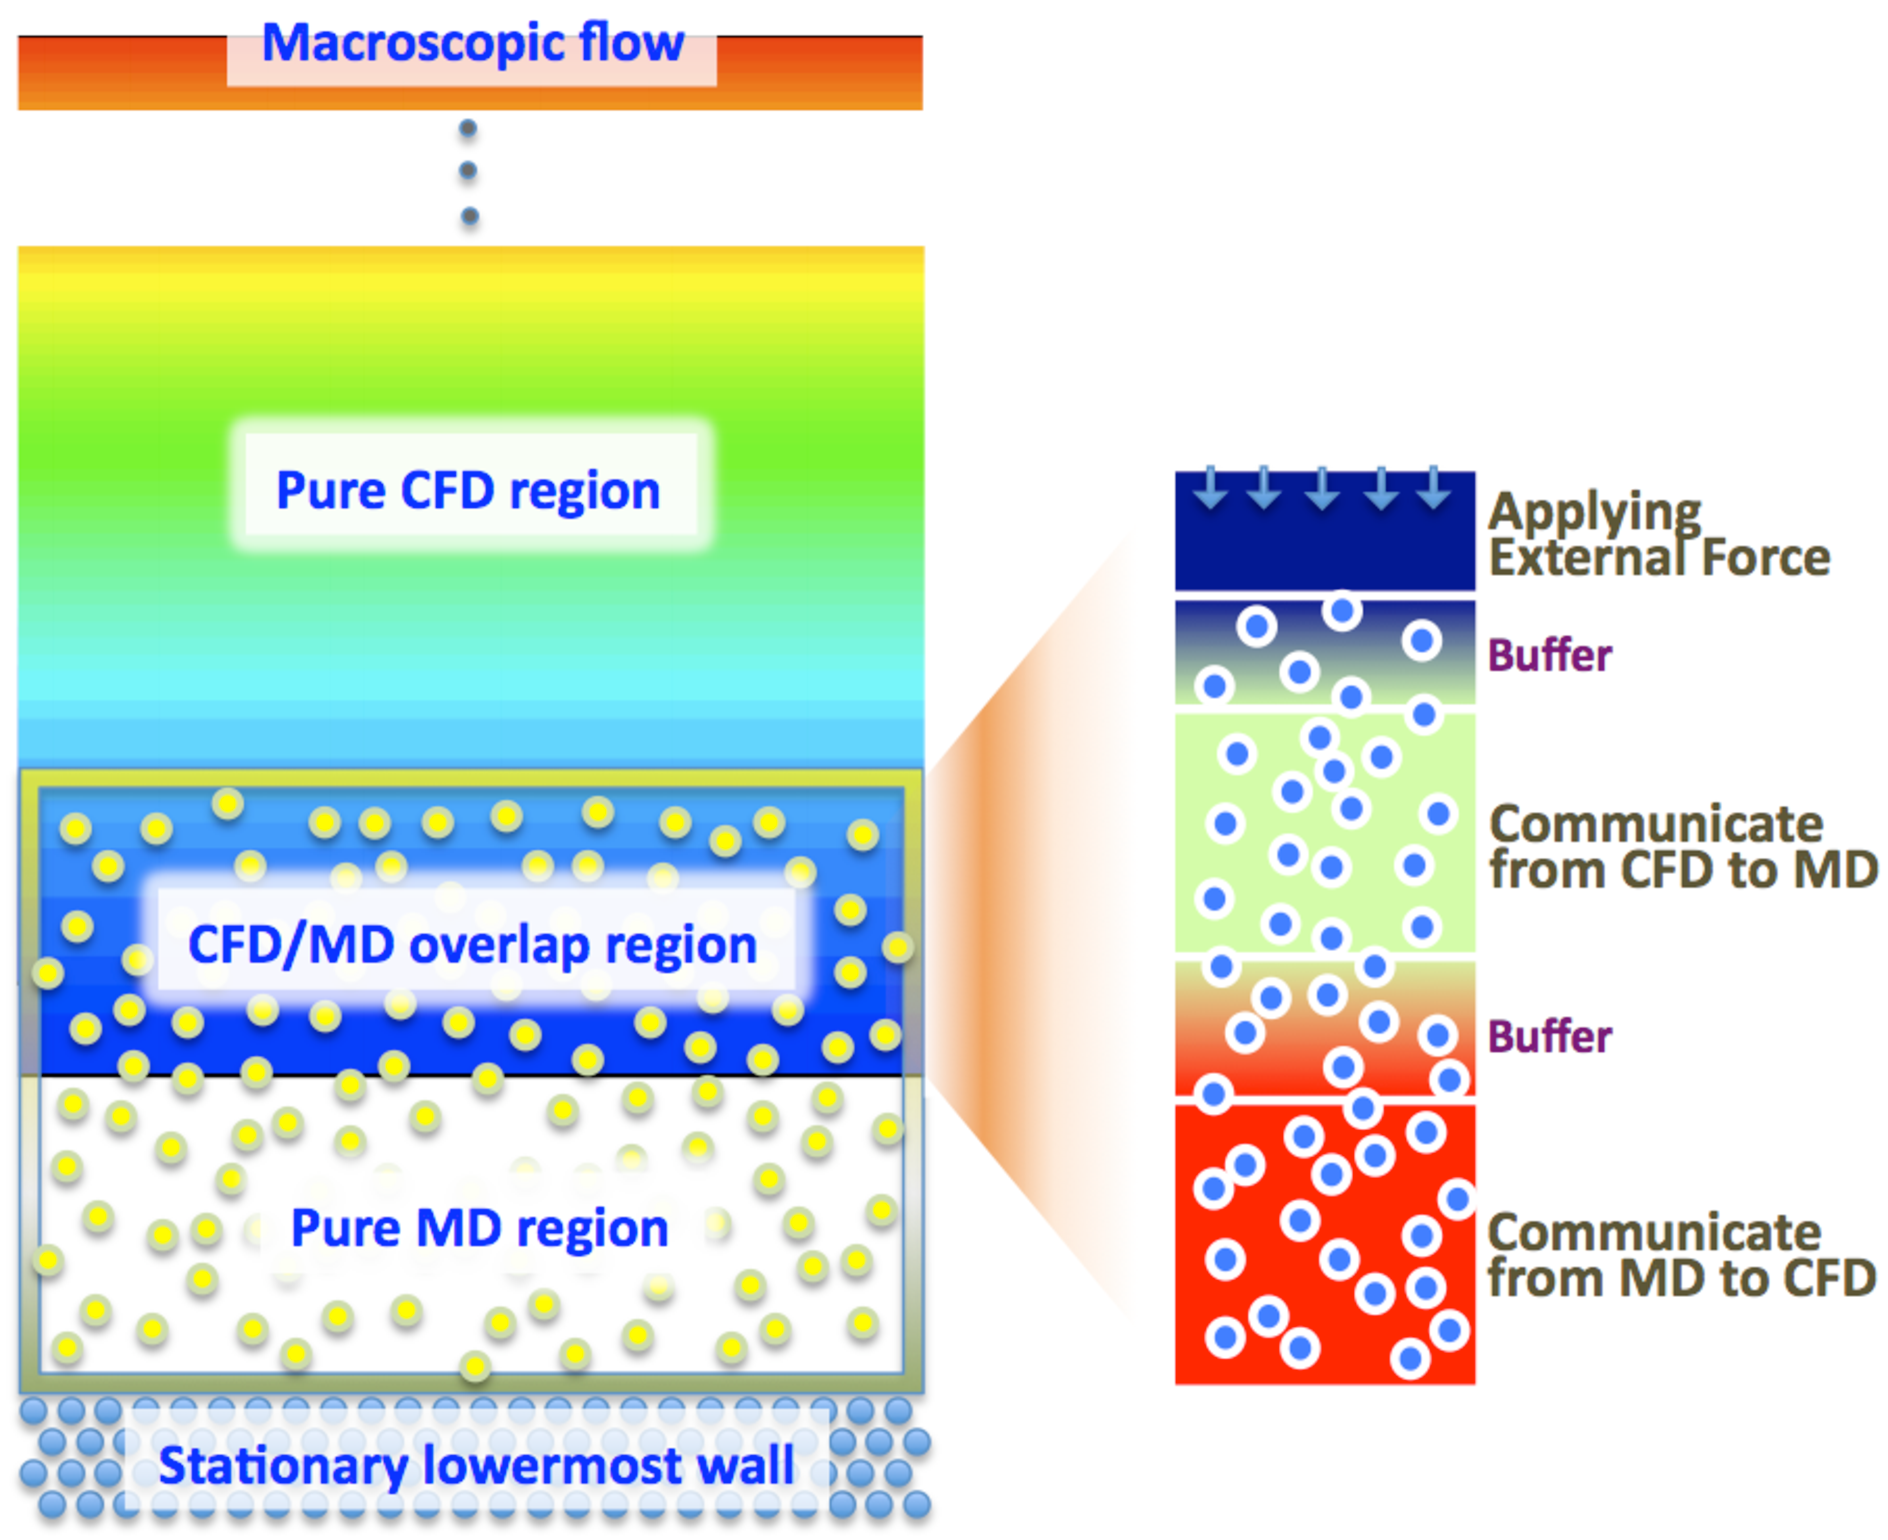
\includegraphics[width=0.8\linewidth]{Hybrid_Schematic.pdf}
\vskip-0.2cm
\caption{\small 
{\bf Schematic Diagram of the Hybrid Domain with Detailed View of Overlapping Zone}
; Overall continuum/atomistic and hybrid computational domain including 
overlap region is presented in the left figure. Detailed layer by layer 
explanation of overlapping region is indicated by the right figure.
}
\label{Fig:Couette}
\vspace{-1em}
\end{figure}


This overlap region is designed sufficiently large to contain five individual layers of sufficient width for the purpose of their existence. The widths of these layers are of course problem dependent. Their roles in the hybrid region are as follows. One layer (the bottom one in Fig. 1-left) provides information from the particle (MD) domain to the continuum one (denoted as ''MDtoCFD''. A second layer (the third one from the bottom in Fig. 1-left) provides information from the continuum domain to the particle one (denoted as ''CFDtoMD''. A third layer (the top one in Fig. 1-left) applies a fictitious external force which prevents particles from escaping from the hybrid domain. These three ''active'' layers are separated by buffer layers, which are placed so as to ensure smooth transitions and that there is no direct correlation between the ''active'' layers. Properties (e.g. velocity) of particles spatially located in the MDtoCFD layer are ensemble-averaged over all the particles in the layer and also averaged over a finite time. The average value is communicated to the continuum solver periodically with a fixed period.

The height of each layer is the same as the CFD cell height and averaged conservative properties in two consecutive layers are passed to continuum domain to be directly imposed as the viscous boundary condition on the Navier-Stokes solver with collocated data structure. The CFDtoMD layer imposes the instantaneous values of properties, velocity in this case, resulting from the continuum solver. This is done via and appropriate constraint to the MD particle-based conservation of momentum on every single particle (constrained dynamics) in the CFDtoMD layer. Thus, particles in this layer are constrained to attain the macroscopic flow property (velocity in this case) on average, while preserving their degree-of-freedom of translational motion. In the uppermost layer, a fictitious external force is exerted on particles to prevent them from escaping the particle domain. This force function is designed to be short-range so as not to be strong enough to influence the motion of the particles past the buffer layer in the CFDtoMD domain. The force stiffens as the particles approach the location where the force becomes infinite in a way that minimizes reflections while preventing the particles from drifting out of the particle domain. The buffer layers existing in between each ''active'' layer are set up to be wider than the interaction length scale of the particles (cutoff radius), in order to prevent direct interaction between particles in neighboring ''active'' layers.



\subsection{Governing Equations and Numerical Schemes}
\label{sec:numerical_schemes}

\subsubsection{Continuum Incompressible Flow Formulation (CFD)}
\label{sec:numerical_CFDschemes}

The current in-house continuum hydrodynamics code solves the unsteady incompressible Navier-Stokes equations: 

\vspace{-.2em}
\begin{eqnarray}
\frac{\partial {u}_{i}}{\partial {x}_{i}} = 0
\end{eqnarray}
\vskip-.6cm
\begin{eqnarray}
\frac{\partial {u}_{i}}{\partial t} + \frac {\partial} {\partial {x}_{j}} ({u}_{i}{u}_{j}) = -\frac {1} {\rho} \frac {\partial p} {\partial {x}_{i}} + \nu \frac {{\partial}^2 {u}_{i}} {{\partial} {{x}_{j}}^2}
\label{eq:NS}
\end{eqnarray}
where $\nu$ is the kinematic viscosity, ${u}_{i}$ denotes the velocity vector, and \textit{p} and $\rho$ expresses pressure and density, respectively.

In this work, the pseudo-compressibility method~\cite{PseudoCompressibility} is adopted to form a hyperbolic system of equations which can be marched in pseudo-time. In this method, an artificial pressure \textit{P} is introduced as $p/\rho$ and the continuity equation is re-written to solve a time derivative of this artificial pressure,

\vspace{-.2em}
\begin{equation}
\frac{\partial P}{\partial t} = - a^2 \frac{\partial {u}_{i}}{\partial {x}_{i}}
 \label{eq:Pseudo}
\end{equation}
where \textit{a} denotes a pseudo-compressibility parameter, currently set up to 3.

For time-accurate unsteady simulation, a dual time stepping method is adopted and it is combined with the LU-SGS (Lower-Upper Symmetric Gauss-Seidel) scheme~\cite{LU-SGS} for the implicit time integration. The inviscid fluxes are upwind-differenced using Osher's flux-difference splitting scheme~\cite{Osher}. For higher-order spatial accuracy, the MUSCL (Monotone Upstream-centered Schemes for Conservation Laws)~\cite{MUSCL} approach is used on an inviscid flux calculation. Viscous fluxes are calculated using conventional second-order central differencing.



\subsubsection{Molecular-Level Formulation (MD)}
\label{sec:numerical_MDschemes}

In MD, an initial velocity is assigned to each atom, and Newton's conservation of momentum is employed at the atomic level to propagate the system's motion through time evolution. In this work the most commonly used Lennard-Jones (12-6) intermolecular force potential model is employed to calculate pair-wise interactions of particles in the system, and is defined as: 

\vspace{-.2em}
\begin{equation}
 u(|r_{i} - r_{j}|) = 4\epsilon_{ij}[(\frac{\sigma_{ij}}{r_{ij}})^{12}-(\frac{\sigma_{ij}}{r_{ij}})^{6}]
 \label{eq:LJ12}
\end{equation}
\normalsize
where  $\epsilon_{ij}$ and $\sigma_{ij}$ denote the pair-wise potential well depth and the atom size parameter respectively, and rij is the distance between the particle i and j. The repulsive term $\it 1/r_{ij}^{12}$ dominating at short rij distance is based on the Pauli principle to avoid overlapping the electronic clouds when particles are very close to each other. The attractive term $\it 1/r_{ij}^{6}$ dominates at long range representing Van der Waals dispersion forces. A cut-off distance $\sigma_{c}$  is introduced here to reduce the computational cost and is set to be 2.2$\sigma$  [28]. Namely when rij exceeds the cutoff the intermolecular force is set to zero without being calculated.
The most common velocity Verlet algorithm is employed for time integration of the equations of motion of the interacting particles and to compute molecular trajectories in the simulation. 
In this work, the MD simulations were performed by using an appropriately modified version of the Large Atomic Molecular Massively Parallel Simulator (LAMMPS). It is a classical molecular dynamics open-source code written in C++ and developed by Sandia National Labs~\cite{LAMMPS_url}.



\subsection{Hybrid Interfaces and Schemes}
\label{sec:numerical_hybridschemes}

Hybrid simulation requires the implementation of hybrid interfaces and schemes based on an individual code. In the current study, the file interface is designed to schedule the information exchange between continuum and discrete particle descriptions. A constrained Lagrangian dynamics model is implemented for hybrid simulation. A unit conversion routine is also implemented in the application code. These changes are summarized in Table~\ref{table:interface_implementation}. 


\begin{table}
  \caption{\small
{\bf Implementation of hybrid interface on CFD and MD codes.} Both codes are equipped with the file-based information exchange routine, to update the hybrid boundary condition. CFD code experiences the global change of its data structure to store the information of the entire fluid system. MD code adopts 
hybrid equations to impose the macroscopic information on microscopic domain and to ensure numerical stability. 
}
  \label{table:interface_implementation}
  \centering
\footnotesize
 \begin{tabular}{>{\centering}p{0.15\textwidth} || p{0.3\textwidth} | p{0.3\textwidth} }
\hline
  & \centering CFD & \multicolumn{1}{c}{MD} \\
\hline
 Global Change & Overset Data Structure (\it{optional}) & \multicolumn{1}{c}{-} \\
\hline
 \centering External Force & \centering - & External Force Equation (Eqn.~\ref{eq:External_Force}) \\
\hline
 \multirow{2}{*}{CFDtoMD} &  \multirow{2}{*}{File Interface: Sender} & {File Interface: Receiver} \\
 & & Constrained MD Equation (Eqn.~\ref{eq:Con3}) \\
\hline
 MDtoCFD & File Interface: Receiver & File Interface: Sender \\
\hline
\end{tabular}
\vspace{-1em}
\end{table}


The CFD code employs the data structure of the overset mesh technique~\cite{Chimera}  to ease the handling of the coupling parameters. In other words, the entire fluid domain is generated because the CFD mesh system and pure MD region is turned off as the ''hole'' cell in the terminology of the overset technique. Likewise, MD to CFD and CFD to MD boundary cells are declared ''fringe'' and ''donor'' cells, respectively. The labor of mesh regeneration due to the change in coupling parameters (the position and depth of the hybrid layers) disappears with the overset data structure.

File-based communicator is employed in both codes. It stores ''donor'' properties on a sender file, monitors the generation of the receiver file from each counterpart and reads the ''fringe'' information. This file interface is scheduled to turn on every sampling interval. The continuum properties are applied to update the constrained Lagrangian dynamics equation in MD solver. The averaged molecular properties are directly imposed as the hybrid CFD boundary conditions. CFD code also takes care of the unit conversion between these distinct codes.
In view of velocity, the CFD solution (non-dimensionalized by the characteristic velocity, e.g., the flat plate velocity in the Couette flow) is converted to the non-dimensional MD unit (molecular characteristic length $\sigma$ divided by the molecular characteristic time $\tau$) before storing the ''donor'' information and vice versa asfer receiving the MD solution.
Regarding the density conversion, we address the relation between the artifical compressibility from CFD and the particle number density from MD by comparing Eq.~\ref{eq:Pseudo} and the original mass conservation equation: 

\vspace{-.2em}
\begin{equation}
\frac{\partial P}{\partial t} = a^2 \frac{1}{\rho} \frac{\partial \rho}{\partial t}
\label{eq:DensityConversion}
\end{equation}

After discretization, we obtain the particle number density in the hybrid CFDtoMD layer as,

\vspace{-.2em}
\begin{equation}
{\rho}_{CM} = \frac {{\rho}_{0}}{1- ({{P}_{CM}-{P}_{0}})/{{a}^{2}}}
\label{eq:NumberDensityCFDtoMD}
\end{equation}
where the subscript \textit{0} denotes initial conditions and subscript \textit{CM} expresses the properties at the CFDtoMD layer.

Likewise, artificial pressure at the hybrid MDtoCFD layer (denoted as the subscript \textit{MC}) is computed from the particle number density as:

\vspace{-.2em}
\begin{equation}
{P}_{MC} = {P}_{0} + {a}^{2} (1- \frac{{\rho}_{0}}{{\rho}_{MC}})
\label{eq:ArtificialPressureMDtoCFD}
\end{equation}


In addition to the file interface, additional constraint equations are employed on the MD code to describe accurately the influence of macroscopic flow variation on the particle domain. First, a fictitious external force should be imposed to prevent the particles from leaving the control domain; the force is applied in the normal direction of the uppermost MD layer. A cost-effective classical external force model by Nie {\it{et al.}}~\cite{Nie} is employed as


\vspace{-.2em}
\begin{equation}
 F_{ext, i} = -p_{a}\sigma\frac{y_{i}-Y_{n-1}}{1-(y_{i}-Y_{n-1})/(Y_{n}-Y_{n-1})}
 \label{eq:External_Force}
\end{equation}
\normalsize
where  $\it p_{a}$ denotes the average pressure in the MD region, $\it Y_{n}-Y_{n-1}$ is the thickness of the uppermost layer to which the force is applied, and $\it F_{ext}$ is the external force acting on ith particle located on position $\it y_{i}$.


Next, at a specific time, the macroscopic flow properties are introduced on the CFDtoMD layer to lead the motion of multiple particles in that layer. The averaged velocity of particles in $\it J_{th}$ cell equals to the velocity $\it u_{J}$ in the continuum cell.


\vspace{-.2em}
\begin{equation}
 u_{J}(t) = \frac {\displaystyle\sum_{i} m_{i} v_{i}} {\displaystyle\sum_{i} m_{i}}
 \label{eq:Con_vel}
\end{equation}
\normalsize
where $\it v_{i}$ is the velocity of the $\it i^{th}$ particle and $\it N_{J}$ is the number of particles in the cell. The Lagrangian derivative of Eq.~\ref{eq:Con_vel} takes the form,

\vspace{-.2em}
\begin{equation}
 \frac{Du_{J}(t)}{Dt} = \frac {\displaystyle\sum_{i} m_{i} \ddot{x_{i}}} {\displaystyle\sum_{i} m_{i}}
 \label{eq:Lagrangian}
\end{equation}
\normalsize

The Classical MD equation of motion can be generalized to obtain the constraint by adopting a perturbation acceleration of each particles, $\zeta_{i}$

\vspace{-.2em}
\begin{equation}
 \frac{F_{i}}{m_{i}} = \ddot{x_{i}}(t)  =   \frac{Du_{J}(t)}{Dt} + \zeta_{i} = \frac{\displaystyle\sum_{i}F_{i}(t)} {\displaystyle\sum_{i}m_{i}} +   \zeta_{i}
 \label{eq:Con2}
\end{equation}
\normalsize
where $\it F_{i}$ is the force on the $\it i^{th}$ particle based on the interactions between particles, $\it m_{i}$ is the mass of each atom and the perturbation acceleration is constrained by,
\vspace{-.2em}
\begin{equation}
\displaystyle\sum_{i}\zeta_{i}m_{i} = 0
 \label{eq:Con2}
\end{equation}
\normalsize


Finally, the constrained particle equation of motion can be written as:


\vspace{-.2em}
\begin{equation}
 \ddot{x_{i}}(t) = \frac{F_{i}}{m_{i}} -  \frac{\displaystyle\sum_{i}F_{i}(t)} {\displaystyle\sum_{i}m_{i}} - \frac{1}{\Delta t_{MD}} \{  \frac{\displaystyle\sum_{i}m_{i}\dot{x_{i}}} {\displaystyle\sum_{i}m_{i}} - u_{J}(t + \Delta t_{MD})\}
 \label{eq:Con3}
\end{equation}
\normalsize



\subsection{Statistical Error and Coupling Parameters}
\label{sec:numerical_noise}

One of the standard issues in obtaining coupled continuum to particle-based (MD) solutions is the fact that the particle-based (MD) solutions have noise, inherent because of limited size of particle ensemble averages and time-sampling limitations. This noise, if not kept under check, is passed on to the continuum solution yielding unphysical results. According to the mathematical expressions in statistical error~\cite{Hadjicon3,Time_Mechanism}, the ratio of sampling noise compared to the macroscopic velocity is inversely proportional to the square root of spatial layer size and temporal sampling duration. For example, reducing the macroscopic velocity by half requires either 4 times larger system domain or 4 times longer sampling to maintain the same order of accuracy. 

Four important coupling parameters determine the scale and pattern of
the sampling noise: The size of sampling layer, its spatial location,
sampling duration and the sampling frequency.
The layer size denotes the volume of a virtual box in which spatial sampling
takes place. The layer location is the perpendicular distance of the sampling
layer from the solid obstacle. The sampling duration ${\Delta}{t_s}$ is denoted as
the time length over which spatially-sampled instantaneous solutions are
accumulated. The sampling interval (inverse of the sampling frequency)
${\Delta}t$ is defined as the time increment between each
hybrid solution exchange.  The layer size and sampling duration
collevtively contribute to the suppression of sampling noise
by increasing the number of sampled particles in space or time.
The layer size is free to be stretched along the periodic direction,
while it results in excessive computational cost. Incresing the layer size
along the non-periodic direction is relatively constrained to secure
the sufficient space for pure CFD and MD domains.
The scale of sampling duration is bound by the sampling interval, which is
desired to be short for accurately describing the temporal variation of 
flow evolution in the unsteady flow field.
The location of the sampling layer also influences the size of fluctuations.
It has been noted that the sampling layer shall be placed sufficiently
far from the solid obstacle to avoid the effect of strong interaction
between fluid and solid particles~\cite{Nie,Yen}.

We take into account the methods of determination of coupling parameters in previous studies~\cite{Nie,Yen,Liu,Hadjicon1,Hadjicon2,Werder,Flekkoy,Delgado1,Time_Mechanism} and intuitively design these parameters considering our application targets. We start from determining the location of the sampling layer according to other previous suggestions, e.g., at least 10$\sigma$ above the bottom wall in the nano-scale liquid argon system. The height of the sampling layer on the non-periodic direction is designed in a way that the sum of pure MD and hybrid regions does not exceed the half of the fluid system. For our deterministic transient/periodic applications, the sampling interval is roughly set to be within 1\% of the transition time or 10\% of the period. The sampling duration is designed the same as the sampling interval.

We also apply the replica sampling approach~\cite{REMD} to supplement the individual hybrid solution. Instead of changing coupling parameters for solving the same fluid system under different flow conditions, we simulate the same coupling configuration with the variance in the initial Maxwell-Boltzmann distribution and average these replicas to find the non-fluctuating solution. In principle, the sampled solution from N replicas has the same order of accuracy as the individual solution from a N-times larger domain. The superiority of replica simulations over a single large-scale simulation can be found from the computational point of view: multiple moderate-sized jobs are more prone to get faster allocation than a single excessive resource requirement on most supercomputing batch queues. Furthermore, this approach is free from the geometric complexity so that it can be applied to the non-periodic three-dimensional flow simulations in which the virtual increase of sampling size is impossible.



\subsection{Temporal Coupling Schemes}
\label{sec:numerical_temporal}

Synchronized and sequential coupling strategies~\cite{Time_Mechanism} are
conventional temporal coupling schemes, which are depicted in
Fig.~\ref{Hybrid_Timescale1}. In synchronized coupling, CFD and MD codes
exchange their hybrid boundary conditions at the same physical time step
and individually evolve by a sampling interval. In constrast, temporal
evolution of each solver takes place one-by-one in sequential coupling,
in a fashion that MD solver advances to the CFD solver by a sampling interval.

The synchronized coupling approach is recommended in view of parallel efficiency.
As can be noticed in the procedure of the sequential approach in
Fig.~\ref{Hybrid_Timescale1}-\subref{sequential_couple},
prossessors statically assigned to an individual task cannot avoid idling
while another code is evolving to the next communication point.
It necessitates the integration of distinct codes to a single MPI executable
or the switching of allocated resource to the active task during runtime.
On the other hand, the synchronized approach introduces the unfavorable
time-lagging phenomenon on CFD boundary condition. As observed in
Fig.~\ref{Hybrid_Timescale1}-\subref{synchro_couple}, molecular dynamic
properties averaged over the backward sampling duration
(from $n{\Delta}t-{\Delta}t_{s}$ to $n{\Delta}t$) represent the CFD
boundary condition at that instance ($n{\Delta}t$).

Wang and He~\cite{Wang} proposed extrapolating hybrid boundary conditions
to resolve the temporal delays in synchronized coupling approach, as seen in
Fig.~\ref{Hybrid_Timescale1}-\subref{synchro_mod}. In their approach,
molecular dynamic time axis is shifted forward by half of the sampling interval
${\Delta}t$ to get rid of the time-lagging event in CFD boundary condition.
Also, MD hybrid boundary condition is imposed by the extrapolated CFD solution
in time. The benefit of this approach is that, in principle,
the time-lagging effect diminishes regardless of the sampling duration.
Thus, the sampling duration can be set as much as the sampling interval.
However, the accuracy of the extrapolated solution is still debatable.
In this scheduling, two \textit{previous} CFD solutions
at $n{\Delta}t$ and $(n-1){\Delta}t$ are extrapolated to predict the
\textit{expected} MD hybrid boundary conditions
from $(n+\frac{1}{2}){\Delta}t$ to $(n+\frac{3}{2}){\Delta}t$.
The extrapolated property is prone to be incorrect from the start
except when the velocity variation is linear in time. In such cases, shortening the sampling
interval ${\Delta}t$ is a way of reducing this extrapolation error. It, in turn, results in
the short sampling duration, which is unfavorable for reducing the statistical error.


\begin{figure}
\centering
\subfloat[Sequential Coupling]{\label{sequential_couple}
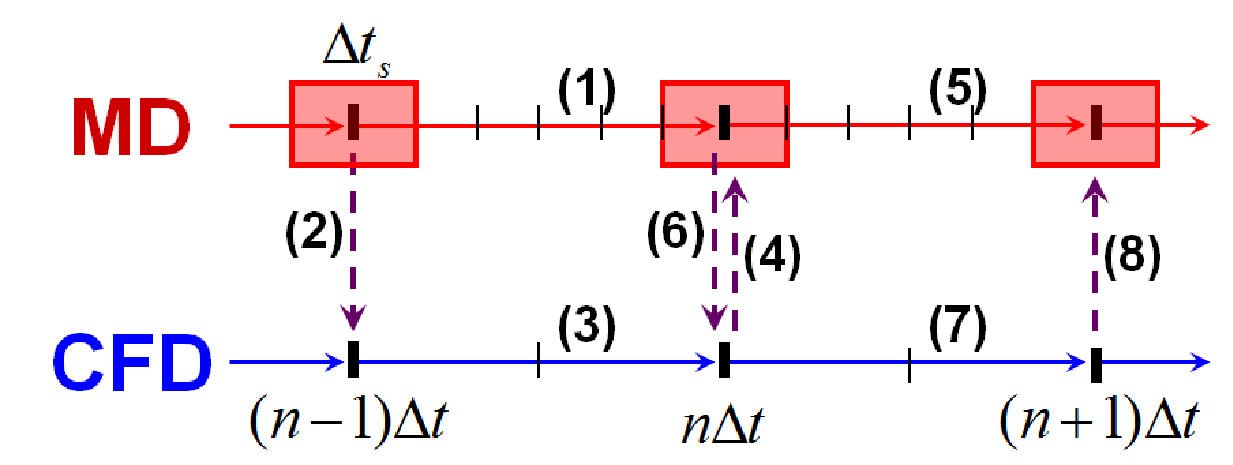
\includegraphics[width=0.7\linewidth]{Sequential_Coupling_Simple.pdf}}
\hskip 1cm
\subfloat[Synchronized Coupling]{\label{synchro_couple}
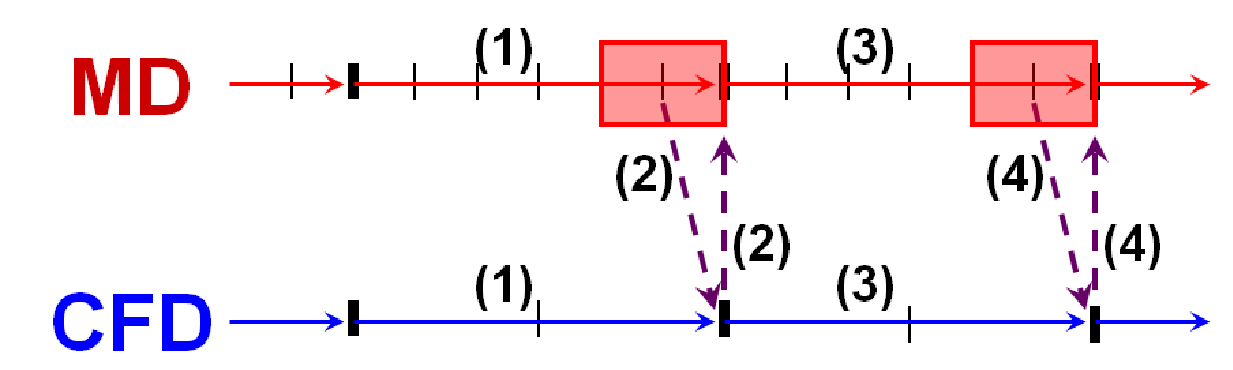
\includegraphics[width=0.7\linewidth]{Synchro_Coupling_Simple.pdf}}
\hskip 1cm
\subfloat[Synchronized Coupling with Extrapolation~\cite{Wang}]{\label{synchro_mod}
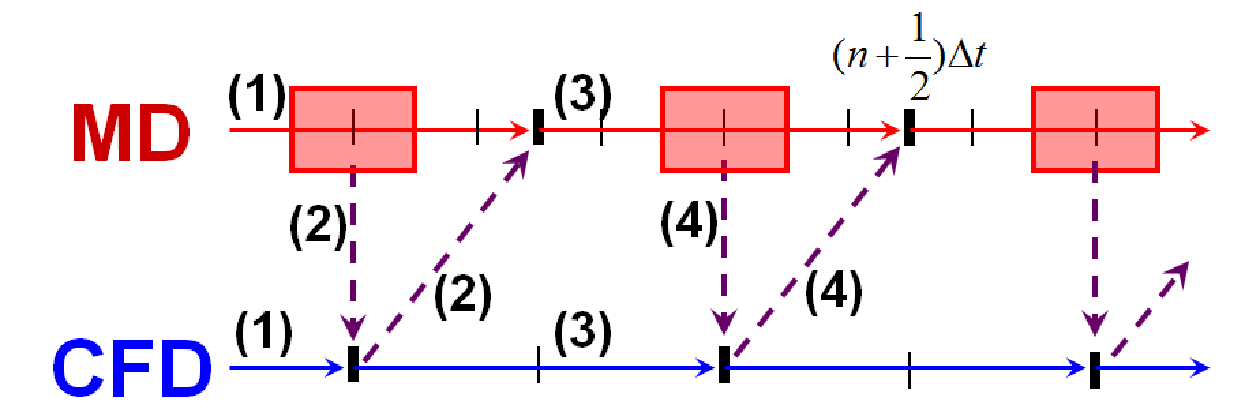
\includegraphics[width=0.7\linewidth]{Prediction_Correction_Org_Simple.pdf}}
\caption[]{\small {\bf Conventional time evolution mechanisms of a hybrid CFD-MD approach.} 
CFD and MD codes are scheduled to conduct data exchange in the overlapping 
region at every $\Delta{t}$ sampling interval.
\subref{sequential_couple} MD code first advances to the next communication
point ($n{\Delta}t$) and passes the centrally-sampled data around
$(n-1){\Delta}t$ to CFD solver so that CFD solver evolves to the $n{\Delta}t$.
One code stays idle while another code evolves.
\subref{synchro_couple} Both codes individually evolve to the communication
point ($n{\Delta}t$) and exchange individual solution.
CFD passes the instantaneous solution at $n{\Delta}t$ while
the backward time-averaged molecular dynamic sample is imposed as the
CFD boundary condition at that time.
\subref{synchro_mod} MD code approaches $(n+\frac{1}{2}){\Delta}t$ while
CFD solver evolves from $(n-1){\Delta}t$ to $n{\Delta}t$. Centrally-sampled MD solution
around $n{\Delta}t$ is supplied as the CFD boundary condition
from $n{\Delta}t$ to $(n+1){\Delta}t$. CFD solution at $n{\Delta}t$ is extrapolated
for the MD boundary condition from $(n+\frac{1}{2}){\Delta}t$ to $(n+\frac{3}{2}){\Delta}t$.}
\label{Hybrid_Timescale1}
\end{figure}


A ''prediction-correction approach'' is designed to reduce this 
extrapolation error by introducing the \textit{predicted} continuum solution at
later time instance, as presented in Fig.~\ref{Hybrid_Timescale2}.
The prediction-correction approach numerically provides non-delayed hybrid
boundary conditions, like Wang and He's formulation. Thus, the sampling
duration is designed as long as the sampling interval.
The main difference from Wang and He's approach is that the CFD code
iterates additional time intervals after it reaches the next communication point.
For example, in Fig.~\ref{Hybrid_Timescale2}-\subref{predcorr_extra},
the CFD code additionally evolves by half of sampling duration after
it approaches $n{\Delta}t$. The CFD code sends these predicted properties
at $n{\Delta}t + \frac{1}{2}{\Delta}{t_s}$ to the MD site and receives the
centrally-sampled molecular dynamic solution around $n{\Delta}t$.
The CFD code rolls back to its previous flow profile at $n{\Delta}t$ and
applies the received molecular dynamic solution to advance to the next
communication point.
A clear benefit of the current approach is that both solvers extrapolate
their boundary conditions from \textit{current} solutions instead of
relying on \textit{previous} history. This advantage eliminates the
sensitivity of the extrapolated solution to the size of the sampling duration,
which enables the increase of the sampling duration to the sufficient level.

The increase of the prediction time scale further increases the accuracy
of the hybrid boundary condition.
In Fig.~\ref{Hybrid_Timescale2}-\subref{predcorr_inter}, the prediction
time scale is increased by one more sampling intervals. While the MD
solver evolves for one sampling interval
from $(n-1){\Delta}t + \frac{1}{2}{\Delta}{t_s}$ to $n{\Delta}t + \frac{1}{2}{\Delta}{t_s}$,
the CFD code runs the actual evolution from $(n-1){\Delta}t$ to $n{\Delta}t$
and adds the predictive evolution for ${\Delta}t + \frac{1}{2}{\Delta}{t_s}$ time
interval. Predicted CFD solution at $(n+1){\Delta}t + \frac{1}{2}{\Delta}{t_s}$
is provided for the interpolated hybrid boundary condition on MD solver.
from $n{\Delta}t + \frac{1}{2}{\Delta}{t_s}$ to $(n+1){\Delta}t + \frac{1}{2}{\Delta}{t_s}$.
Figure ~\ref{Hybrid_Timescale2}-\subref{predcorr_both} demonstrates the
imposition of implicit boundary conditions on both domains. In this formulation,
CFD time is shifted backward by one sampling interval and the prediction step
is scheduled as $2{\Delta}t + \frac{1}{2}{\Delta}{t_s}$.


\begin{figure}
\centering
\subfloat[Extrapolated Hybrid Boundary Conditions]{\label{predcorr_extra}
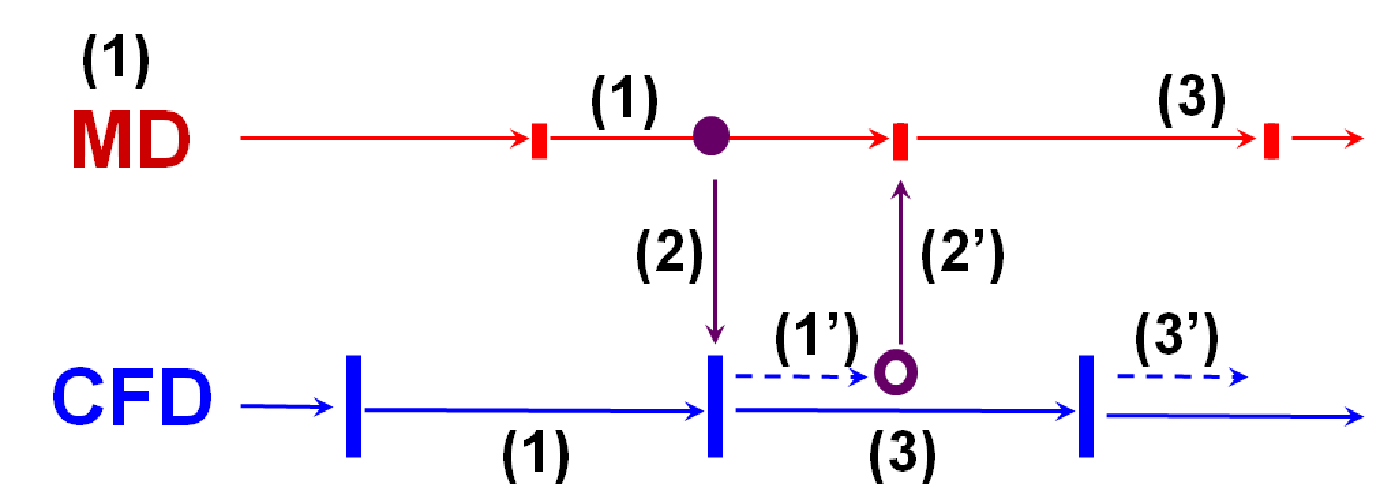
\includegraphics[width=0.7\linewidth]{Prediction_Correction_Extra_Simple.pdf}}
\hskip 1cm
\subfloat[Interpolated MD Boundary Condition]{\label{predcorr_inter}
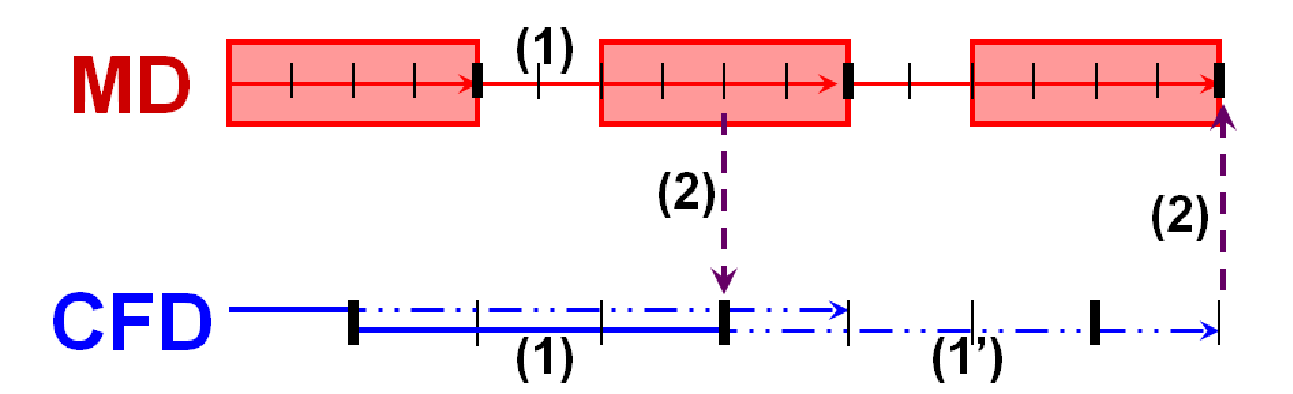
\includegraphics[width=0.7\linewidth]{Prediction_Correction_Inter_Simple.pdf}}
\hskip 1cm
\subfloat[Interpolated Hybrid Boundary Conditions]{\label{predcorr_both}
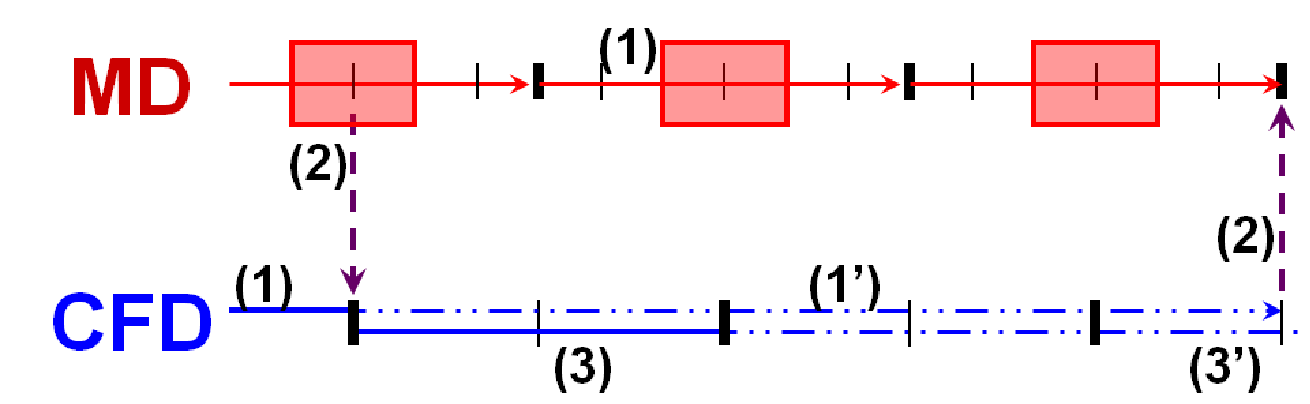
\includegraphics[width=0.7\linewidth]{Prediction_Correction_Both_Simple.pdf}}
\caption[]{\small {\bf A prediction-correction approach with extrapolated / interpolated hybrid boundary conditions.} 
\subref{predcorr_extra} While MD code evolves for one sampling interval from
$(n-1){\Delta}t + \frac{1}{2}{\Delta}{t_s}$, CFD solver runs the actual evolution
from $(n-1){\Delta}t$ to $n{\Delta}t$ and adds the the prediction step
for $\frac{1}{2}{\Delta}{t_s}$. MD code gets the \textit{predicted} continuum hybrid solution
at $n{\Delta}t + \frac{1}{2}{\Delta}{t_s}$ while CFD solver receives the
centrally-sampled MD data around $n{\Delta}t$. Both codes extrapolate received solutions
for imposing hybrid boundary conditions for the next evolution loop.
\subref{predcorr_inter} The prediction step in CFD solver is increased to
${\Delta}t + \frac{1}{2}{\Delta}{t_s}$. MD code interpolates two \textit{predicted}
CFD solutions at $n{\Delta}t + \frac{1}{2}{\Delta}{t_s}$ and
$(n+1){\Delta}t + \frac{1}{2}{\Delta}{t_s}$ for the hybrid boundary conditions
when the code evolves over the same interval.
\subref{predcorr_both} Time axis of CFD domain shifts backward by 1 sampling
interval and the prediction step is set $2{\Delta}t + 0.5{\Delta}{t_s}$.
Hybrid boundary conditions at both solvers are acquired through the interpolation.}
\label{Hybrid_Timescale2}
\end{figure}


The current numerical approach provides more accurate time-variant solution
by decreasing or eliminating the unfavorable overshoot/undershoot phenomena
in extrapolations. Nevertheless, an additional computational cost is inevitable
for the CFD simulation. Thus, the current approach is applicable to the problems
in which computational cost on CFD is quite smaller than that of MD simulation.



\section{Coupled Concurrent Multi-Scale (Continuum-Molecular) Simulation Framework}
\label{sec:computational}

Two important issues regarding the performance of hybrid simulations are co-scheduling and load balancing. Both can be resolved by adopting the Pilot-job concept. We explain the design of a multi-physics simulation framework that operates in the form of a single Pilot-job and contains a load-balancing function between distinct tasks.

\subsection{SAGA and SAGA-based Frameworks - An Efficient Runtime Environment for Coupled Multi-component Computations}
\label{sec:computational_SAGAandBigJob}

The simple API for grid applications (SAGA)~\cite{saga_url} is an API standardization effort within the open grid forum (OGF)~\cite{ogf_web}, an international standards development body concerned primarily with standards for distributed computing. SAGA provides a simple, POSIX-style API to the most common grid functions at a sufficiently high-level of abstraction in order to be independent of diverse and dynamic grid environments. The SAGA specification defines interfaces for the most common grid-programming functions grouped as a set of functional packages (Fig.~\ref{Fig:SAGA1}). Some key packages are the following:


\begin{figure}
 \begin{center}
     \includegraphics[width=0.8\textwidth]{Structure_of_SAGA.eps}
 \end{center}
\caption{\small {\bf Layered schematic of the different components of the SAGA landscape.} At the topmost level is the simple integrated API which provides the basic functionality for distributed computing. Our BigJob abstraction is built upon this SAGA layer using Python API wrapper}
 \label{Fig:SAGA1}
 \vspace{-1em}
\end{figure}

\begin{itemize}
\item File package - provides methods for accessing local and remote file systems, browsing directories, moving, copying, and deleting files, setting access permissions, as well as zero-copy reading and writing
\item Job package - provides methods for describing, submitting, monitoring, and controlling local and remote jobs. Many parts of this package were derived from the largely adopted DRMAA %~\cite{drmaa_url} specification.
\item Stream package - provides methods for authenticated local and remote socket connections with hooks to support authorization and encryption schemes.
\item Other Packages, such as the RPC (remote procedure call) and Replica package
\end{itemize}


BigJob~\cite{repex_ptrsa} is a SAGA-based Pilot-Job application, by which a number of sub-tasks can run in a pre-defined schedule with the specified number of processors whether or not they are coupled. We devised this solution to overcome the concurrent scheduling requirement of coupled CFD and MD jobs and to allocate resources for the load balancing of these codes. The advantage of the BigJob application over other Pilot-Job implementations is that it is infrastructure-neutral, thanks to various adaptors in SAGA.

Fig.~\ref{Fig:BigJob_Structure}  shows the structure of BigJob and its operation flow. When a BigJob item is submitted to the remote resource, the application manager monitors the status of this Pilot-Job through the advert service. When resources are allocated to BigJob, the application manager allots the obtained resources to its sub-jobs, and a coupled simulation starts under the control of a multi-physics agent in the remote resource. The advert service is constantly notified about the status of a Pilot-Job from the queuing system and the status of sub-jobs from the multi-physics agent. It also delivers this information to the application manager by a push-pull mechanism. The application manager watches the status of the sub-jobs and, when the coupled simulation is finished, decides on the next event. If an individual simulation is of interest, the manager closes the BigJob allocation when the simulation is finished. In cases of multiple replica simulations or load-balanced coupled simulation, the manager re-launches the sub-jobs on the same BigJob allocation until all replicas or simulation loops are completed.


\begin{figure}
\centering
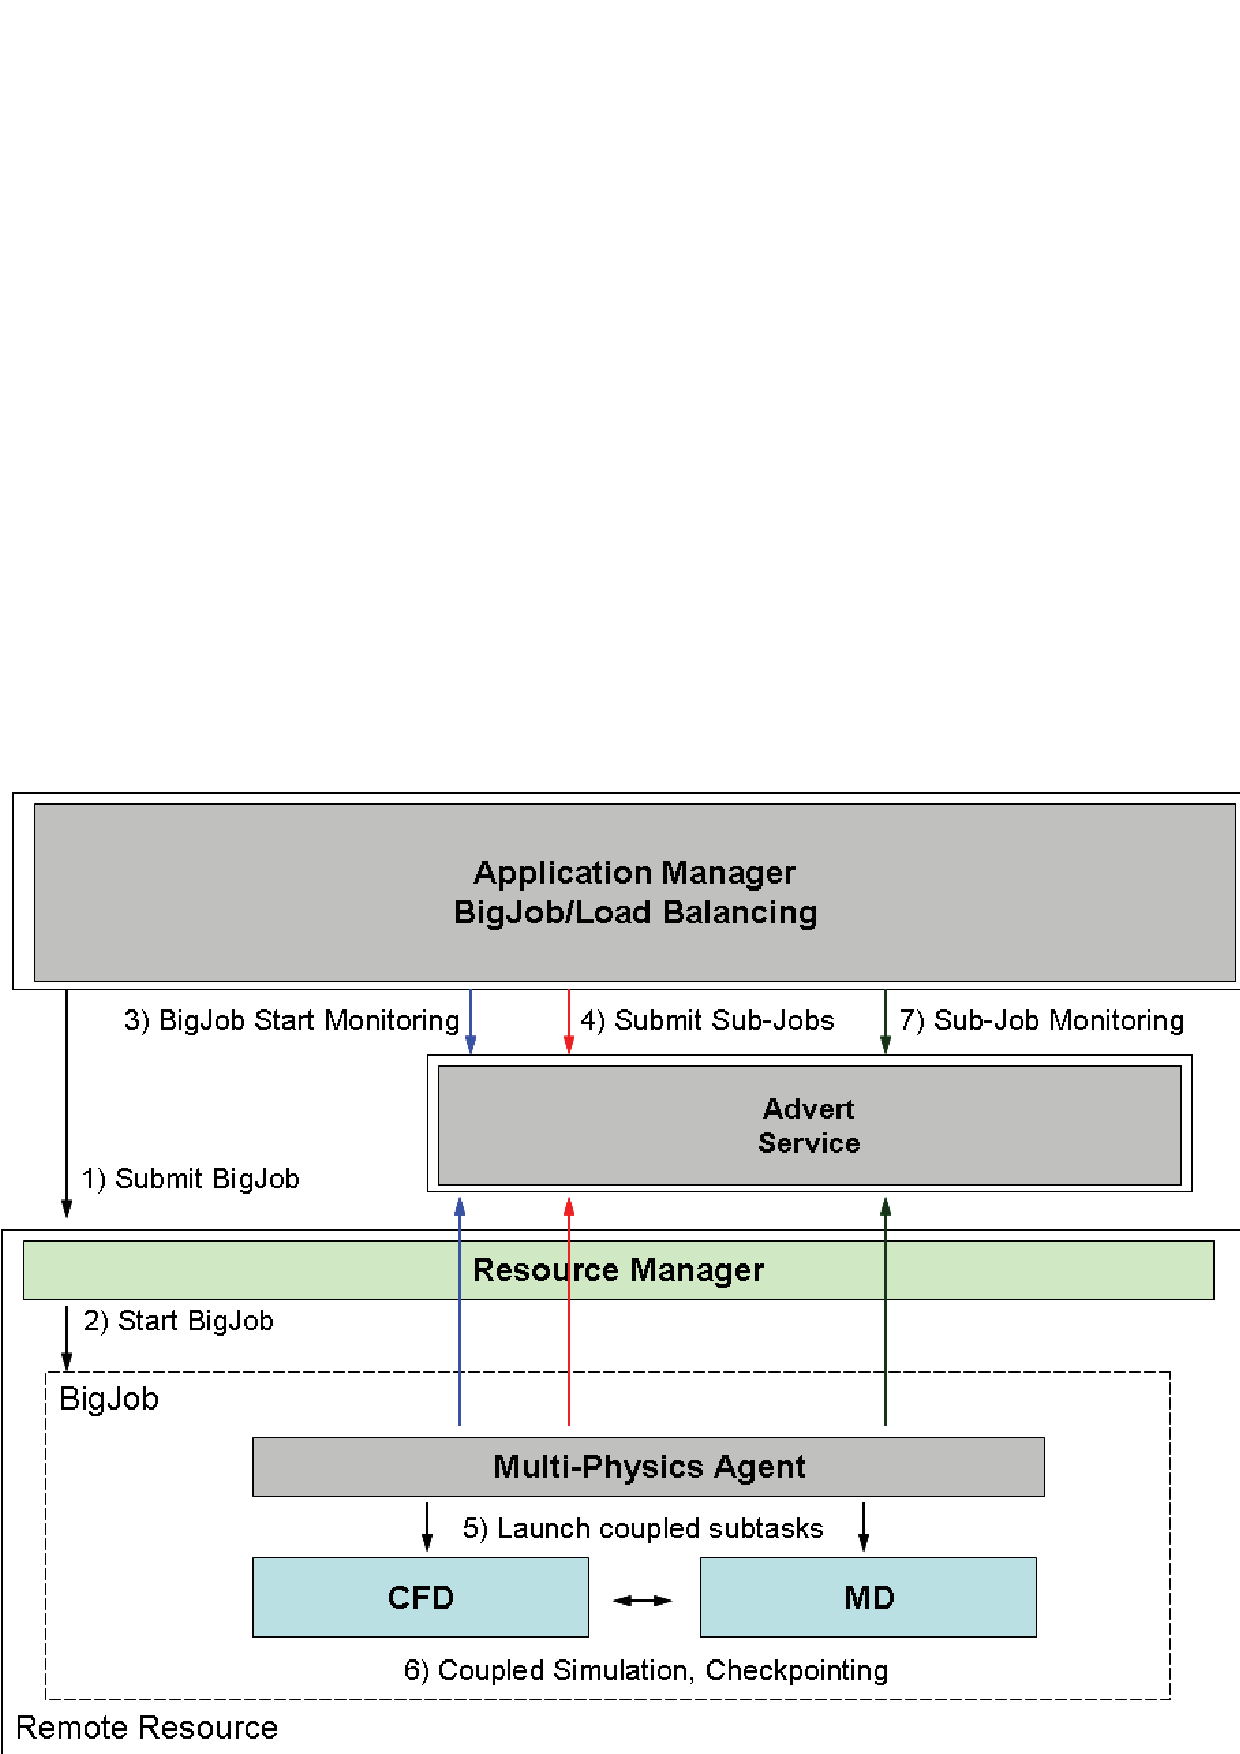
\includegraphics[width=0.8\linewidth]{Structure_of_BigJob}
\caption{\small {\bf Architecture of the controller/manager and control flow.} The application manager is responsible for job management including BigJob and sub-job submission, their status monitoring functions. We implement a load-balancing module, and migration service based on job information. The application agent system resides on each HPC resource and conducts job information gathering and also communicates with the application manager via the advert service}
\label{Fig:BigJob_Structure}
\vspace{-1em}
\end{figure}



\subsection{Load-Balancing of Coupled Multi-Physics Simulation}
\label{sec:computational_LoadBalancing}
The load-balancing of a coupled simulation implies sufficient flexibility to re-distribute resources to an individual job according to each performance. We will discuss the implementation and algorithm of a simple load balancer (LB)~\cite{Ko}; it is important to mention that the LB functions in the context of the SAGA-BigJob framework.

The idea is to assign more resources to heavier sub-jobs under the fixed resource allocation, until all sub-jobs elapse at the same execution time. As it is impossible to predict the performance of each code in advance, we let the LB monitor the wall-clock time between the information exchange points of the coupled sub-jobs and iteratively change the resource distribution until load-balancing is achieved. As the individual solver is considered as black-box, each application code is assumed to have the ideal parallel efficiency. In case the application codes are highly scalable, the LB can find the best condition after a few dynamic re-distributions. In addition, all processors in one node are assigned to one single task to prevent the interference (and performance degradation) observed when multiple MPI tasks share the node.

Let the computation time (between exchanges) of the two sub-jobs are $t_{CFD}$ and $t_{MD}$, and the number of cores assigned to each domain being $PE_{CFD}$ and $PE_{MD}$, respectively. Subscripts C and N denote current and next states. Assuming ideal parallel efficiency, the total load of each application remains the same after resource re-allocation,


\vspace{-.2em}
\footnotesize
\begin{eqnarray}
W_{CFD}&=&PE_{CFD,C}\times t_{CFD,C}=PE_{CFD,N}\times t_{CFD,N} \nonumber \\
W_{MD}&=&PE_{MD,C}\times t_{MD,C}=PE_{MD,N}\times t_{MD,N}
\label{eq:SimTime_EachTask}
\end{eqnarray}
\normalsize


In spite of the re-allocation, the total number of cores utilized remains the same:


\vspace{-.2em}
\footnotesize
\begin{equation}
PE_{TOT}=PE_{CFD,C}+PE_{MD,C}=PE_{CFD,N}+PE_{MD,N}
\label{eq:PECondition}
\end{equation}
\normalsize


Our objective is to reduce the computation time of a sub-job to the point where the two application components show the same computation between the exchange points, i.e., $t_{CFD,N} = t_{MD,N}$. Derived from Eqn.~\ref{eq:SimTime_EachTask} and Eqn.~\ref{eq:PECondition} the optimal number of cores distributed for the CFD sub-job would be:


\vspace{-.2em}
\footnotesize
\begin{eqnarray}
PE_{CFD,F} & = & \frac {W_{CFD}} {(W_{CFD} + W_{MD})} \times PE_{TOT}
\end{eqnarray}
\normalsize

The MD simulation (sub-job) will follow a similar expression.

The above non-integer values proceed in discrete values expressed as the multiples of the number of CPU cores in a node. We chose the nearest discrete number to our load-balancing as the optimal number of processors in each application.



\subsection{Implementation of an Execution Framework and Application-level Corrections}
\label{sec:computational_hybridruntime}

A hybrid CFD-MD framework is evaluated by implementing the application manager shown in Fig.~\ref{Fig:BigJob_Structure}, which is written in PYTHON script language. By default, an application manager calls a number of SAGA functions in sequence, to allocate a vacant job, to run individual MPI simulations, to monitor its status, and to finalize the BigJob allocation.

In the case that the load-balancing capability is turned on, the situation becomes complicated. A single MPI job is not able to change its number of processors during the simulation, which implies that coupled codes should stop-and-restart to be assigned with the changed number of processors. Thus, sub-jobs are scheduled to have multiple restarts from the previous check-pointing solution, which we denote ''simulation loop''. An LB is provided as a separate function in an application manager and is scheduled to run in between each restart of the sub-jobs.

The efficient functioning of the LB is predicated on application codes being able to restart effectively from their check-pointing data. Application codes should also be equipped with a generalized domain partitioning routine to run a simulation with any number of processors without harming their parallel efficiency. Another change implemented in the application codes is the time checking routine. The runtime of each application is meaningless in running a LB since this runtime contains idle waiting on the inter-domain information exchange as well as the individual simulation time. The actual runtime can be counted by putting a wall-time function before and after the information exchange routine.

The generation of an application manager and the changes in application codes raise the possible simulation scenarios shown in Fig.~\ref{Fig:OneBJ_Flow}. The first (extreme left) scenario shows the time evolution of a coupled simulation under a conventional job submission (which we defined as scenario S0), and others using a BigJob application (denoted as S1). For S0, individual tasks with resource requirements of $PE_{CFD}$ and $PE_{MD}$, respectively, are independently submitted to the conventional queuing system, and the job scheduler recognizes these coupled tasks as two distinct jobs. Thus, on average, they start at different times. In this case, both tasks wait in the queue when no job is allocated (waiting stage). The first allocated job idles to perform data exchange with its counterpart (idling stage), and the actual simulation starts when both jobs are allocated (running stage). On the other hand, for scenario S1, a BigJob of size $PE_{CFD}+PE_{MD}$ is submitted to the queue, and coupled simulation directly starts when the resource is assigned to this BigJob. Because of the co-scheduling of sub-jobs, a BigJob is free from a long inactive mode, which is frequent in conventional job submission, while the total runtime is the same if the resource distribution to the sub-jobs is identical. However, eliminating the inactive mode in itself does not guarantee a reduction in the total runtime because a larger single allocation may result in a greater queue waiting time than that when two simulations request a smaller number of processors each (but with the same total). The same situation can arise for the load-balanced case with one BigJob (S1\lb). From the comparison between S1 and S0, we can estimate the performance gain by the concurrent start of distinct coupled codes. Compared with other scenarios, the S1\lb solution demonstrates the benefit of a load-balancing function on coupled simulations.


\begin{figure}
\centering
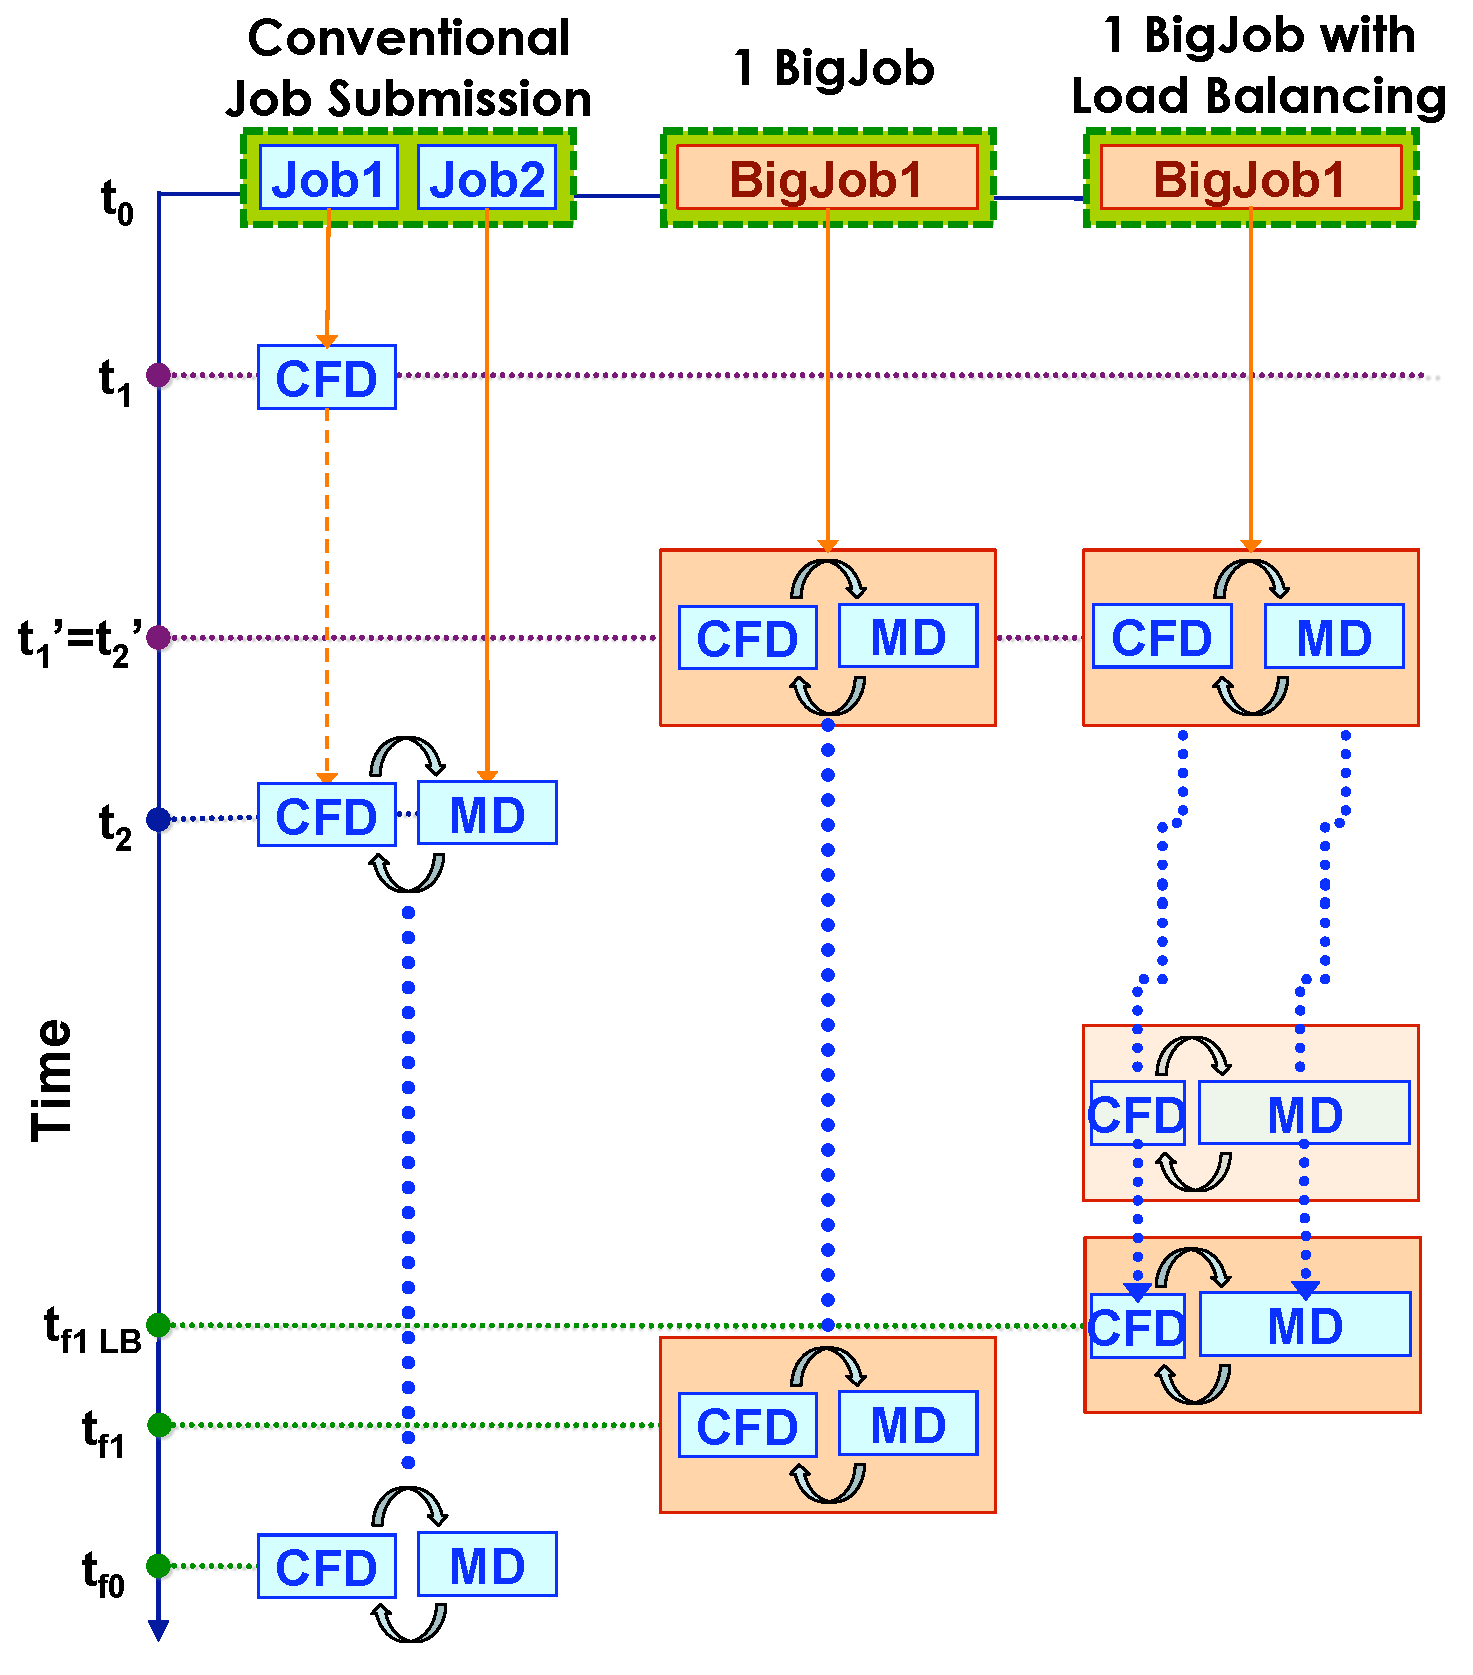
\includegraphics[width=0.8\linewidth]{Single_BigJob_Scenarios_new.pdf}
\caption{\small {\bf Comparison of dependencies encountered for coupled
  simulations submitted as conventional jobs, to the scenario when
  using Pilot-Jobs.} Here we use only 1 BigJob (S1). The conventional
  mode of submission experiences three phases based upon their queue
  state: (i) All jobs are waiting: ($t_1-t_0$); (ii) Inactive mode
  (where one job is waiting for another: $t_2-t_1$), and (iii) Active
  mode (running a coupled simulation: $t_f-t_2$). The Inactive stage,
  disappears when a coupled simulation runs within a BigJob, as an
  allocated BigJob distributes its resource to both sub-jobs.}
\label{Fig:OneBJ_Flow}
\vspace{-1em}
\end{figure}



\section{Multi-physics Flow Simulations in Various Flow Conditions}
\label{sec:accuracy}
A hybrid CFD-MD framework is employed to solve a nano-scale multi-physics flow field. We solve the transient Couette flow and the oscillating boundary problem, to evaluate the capability of solving moderate-speed flow field and to verify a ''prediction-correction''  temporal coupling scheme. 

\subsection{Problem Description and Coupling Conditions}
\label{sec:accuracy_conditions}
Both the Couette flow and oscillating boundary problems solve the same geometric configuration of a nano-scale channel which is filled with liquid argon. The characteristic length of liquid argon is ${\sigma} =3.405{\times}10^{-10}$ and the time scale is  $\tau=2.2{\times}10^{-12}$. The density is 0.81${\sigma}^{-3}$, which implies that 0.81 atoms are placed in the characteristic volume. Wall materials are artificially designed to have the same characteristics as the liquid argon particle. The slip ratio between fluid and solid particles is set at 0.6 to satisfy the linear velocity gradient along a vertical direction~\cite{Nie}. The channel is 52$\sigma$ in height, which is  O(10$^{-8}$)  meters. Applications covered in this work are periodic systems in a perpendicular direction, and the flow is derived by the horizontal motion of the upper plate. 

The computational domain for the hybrid simulation is depicted in Fig.~\ref{Couette_Val_Domain}. The pure MD region is specified as 10$\sigma$, which was reported to be sufficient to prevent strong fluctuation between fluid particles and wall materials from direct transportation to CFD domains~\cite{Yen}. The hybrid region is designed to be 16$\sigma$ to guarantee that the molecular simulation domain does not exceed the half of the fluid system. The hybrid region is divided into 8 layers. Two layer boundary zones from the particle to the continuum domain are placed ahead of the pure MD region, from 10 to 14$\sigma$. Two layers of the continuum domain to the particle boundary are positioned from 18 to 22$\sigma$ and the external force region is placed at the top of hybrid region, from 24 to 26$\sigma$. Both the sampling interval and the sampling duration are set to be 10$\tau$, considering the characteristics of our deterministic application targets. Finally, the width of the MD domain along the periodic direction is determined at 140$\sigma$, after a number of numerical experiments. 

%Both the Couette flow and oscillating boundary problems solve the same geometric configuration of a nano-scale channel which is filled with the liquid argon. The characteristic length of the liquid argon is ${\sigma}=3.405{\times}10^{-10}$ and the time scale is $\tau=2.2{\times}10^{-12}$. The density is $0.81m{\sigma}^{-3}$, which implies that 0.81 atoms are placed in the characteristic volume. Wall material is the \textit{frozen} argon particle with the same density as the fluid system. The slip ratio between fluid and solid particles is set at 0.6 to satisfy the linear velocity gradient along a vertical direction.~\cite{Nie} The channel is 52 $\sigma$ in height, which is O(10$^{-8}$) meters. Applications covered in this work are periodic systems along the horizontal direction, and the flow is derived by the horizontal motion of the upper plate.

%The computational domain for the hybrid simulation is depicted in Fig.~\ref{Couette_Val_Domain}. The pure MD region is specified as 10 $\sigma$ from the bottom of the wall. According to Yen \textit{et al.}~\cite{Yen}, this is the reasonable distance to avoid the direct influence of the strong fluctuation between fluid particles and wall materials on molecular samples at the hybrid MDtoCFD layer.
%The hybrid region is composed of 8 sublayers each with 2 $\sigma$ along the vertical direction. Two layer boundary zones from the particle to the continuum domain (MDtoCFD layers) are placed ahead of the pure MD region, from 10 to 14 $\sigma$. Two layers of the continuum domain to the particle boundary (CFDtoMD layers) are positioned from 18 to 22 $\sigma$ and the external force region is placed at the top of hybrid region, from 24 to 26 $\sigma$. Two buffer layers from 14 to 18 $\sigma$ and one buffer layer from 22 to 24 $\sigma$ are added between these active layers.
%Both the sampling interval and the sampling duration are set to be 10 $\tau$, considering the characteristics of our deterministic application targets. Finally, the width of the MD domain along the periodic direction is determined at 140 $\sigma$, after a number of numerical experiments.


\begin{figure}
\centering
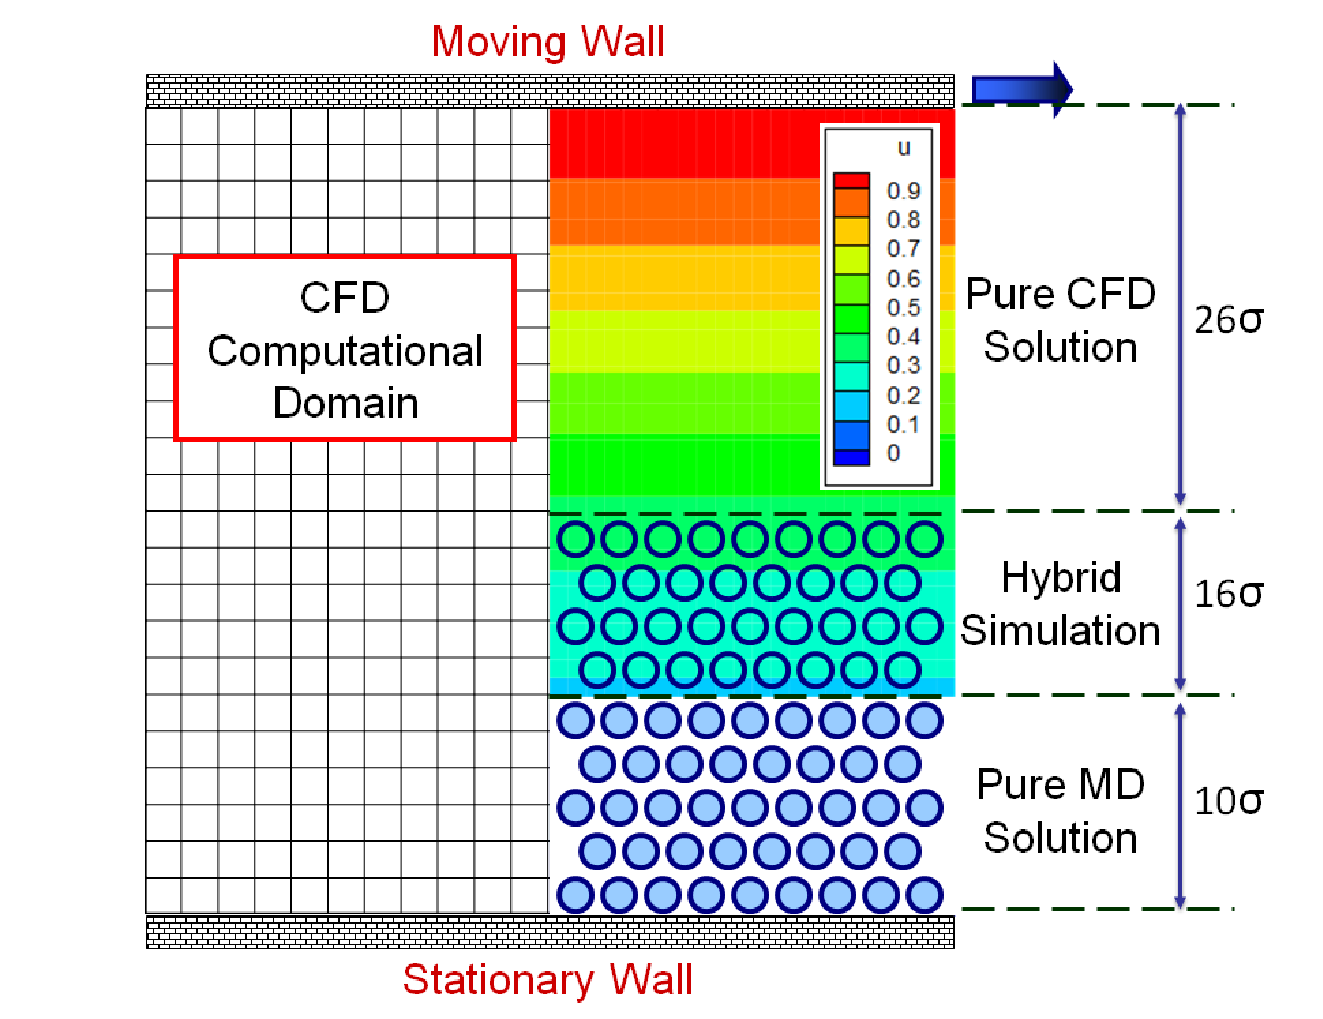
\includegraphics[width=0.8\linewidth]{Couette_Val_Domain.pdf}
\vskip-0.2cm
\caption{\small {\bf Computational domain of the Couette flow simulation.} The height of the fluid domain is 52$\sigma$ ($\approx$177$\AA$). CFD mesh size is 71$\times$27 and CFD cells at the pure MD region are treated as holes. MD domain size is about 140$\sigma$ in the X-direction and around 26$\sigma$ in the Y-direction, including the bottom wall. A Periodic boundary condition is applied on the principal flow direction.}

\label{Couette_Val_Domain}
\end{figure}



\subsection{A Transient Couette Flow}
\label{sec:accuracy_couette}

%A transient Couette flow is simulated to verify the accuracy of the current framework with a multiple replica sampling approach for the moderate-speed flow simulation. This application has been widely used for the validation of a hybrid CFD-MD solver~\cite{Nie,Yen}. The flow is initially set at stationary and the upper wall starts the horizontal motion with a constant velocity (1 $\sigma$/$\tau$). Figure~\ref{Flat_Plate_Sol} presents transient Couette flow profiles by CFD, MD, and hybrid simulations. Pure CFD produces the identical result as the analytic solution: Pure MD also describes the same flow profile with the slight sampling noise. These results verify the accuracy of the individual solver. The hybrid simulation also provides the same flow profile, again with the slight deviation due to the fluctuation in the sampled MD property. It proves that the current hybrid framework accurately analyzes the steady flow field in nano-scaled systems.

A transient Couette flow is simulated to verify the accuracy of the current framework with a multiple replica sampling approach for the moderate-speed flow simulation. This test problem has been widely used for the validation of hybrid CFD-MD solvers~\cite{Nie,Yen}. The initial condition for the simulation is with the fluid between the plates at rest in the CFD domain. In the particle domain at the lower wall, the initial state is reached by providing initial positions for the fluid particles (atoms) and then solving the equations of motion without the constraints imposing motion with non-zero mean velocity, but maintaining the ?etaining?force (eq. ~\ref{eq:LJ12}). An instantaneous state resulting from this simulation is then used as the initial condition for the MD part of the hybrid simulation after statistical equilibrium has been reached. The hybrid simulation is started by imposing a horizontal velocity  of  (1 $\sigma$/$\tau$) as the upper wall boundary condition to the CFD solver. Figure~\ref{Flat_Plate_Sol} presents simulation results of transient Couette velocity profiles obtained by CFD, MD, and hybrid simulations. Pure CFD produces virtually identical results as the analytical solution with no-slip boundary conditions as expected based on the definition of the problem, which was done to ensure the validity of both the continuum and MD formulations. The pure MD and hybrid solutions are also in good agreement with the analytical solution to within the sampling statistical uncertainty in the calculation of average velocities.

These results validate the individual solvers as well as the CFD-MD coupling scheme for the hybrid simulation. They also indicate that the current hybrid framework adequately represents the steady flow field in this nano-scale system. 


\begin{figure}
\centering
\subfloat[Pure CFD and MD Results]{\label{cfd_md_couette}
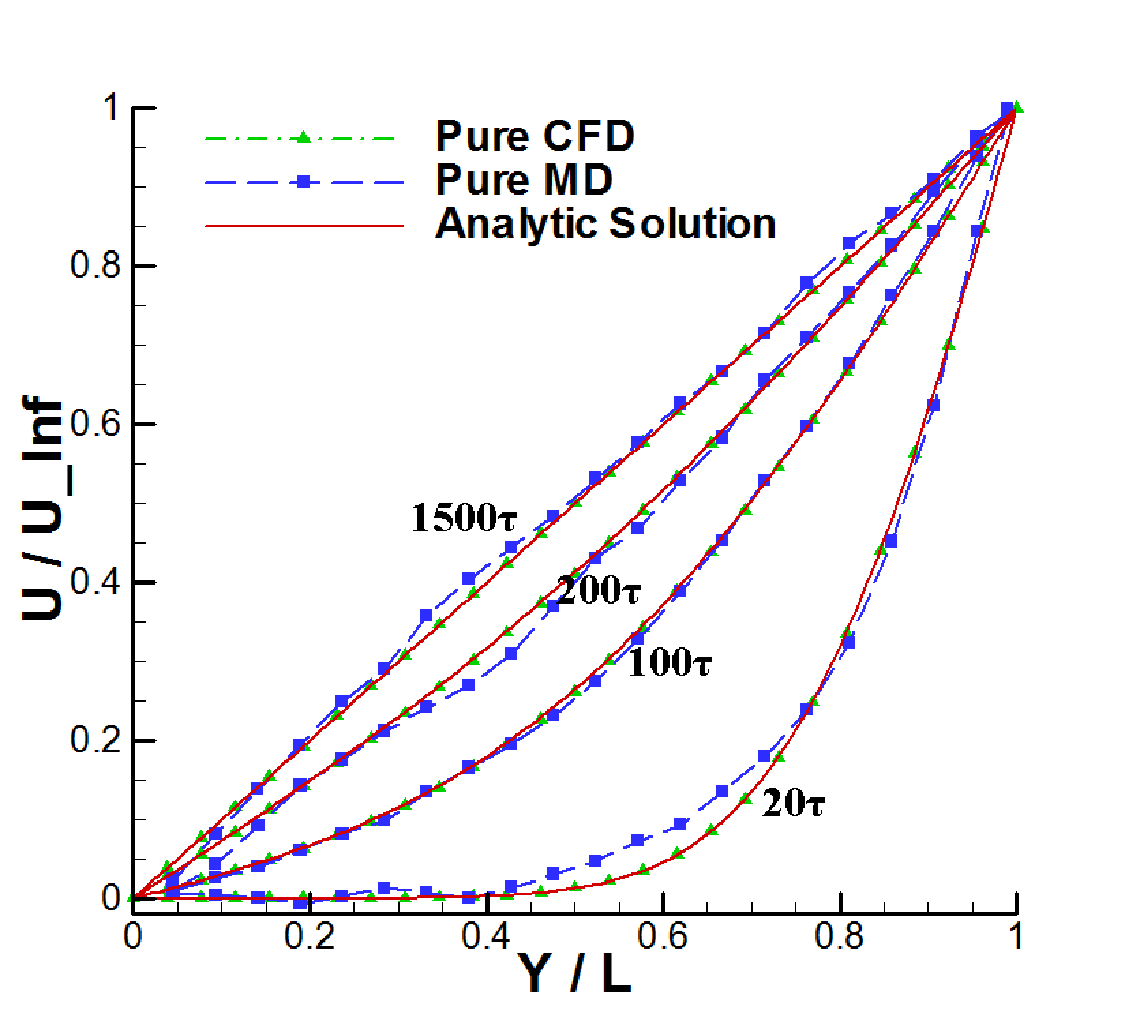
\includegraphics[width=0.6\linewidth]{Flat_Plate_Sol1.pdf}}
\hskip 1cm
\subfloat[Hybrid CFD-MD Solution]{\label{hybrid_couette}
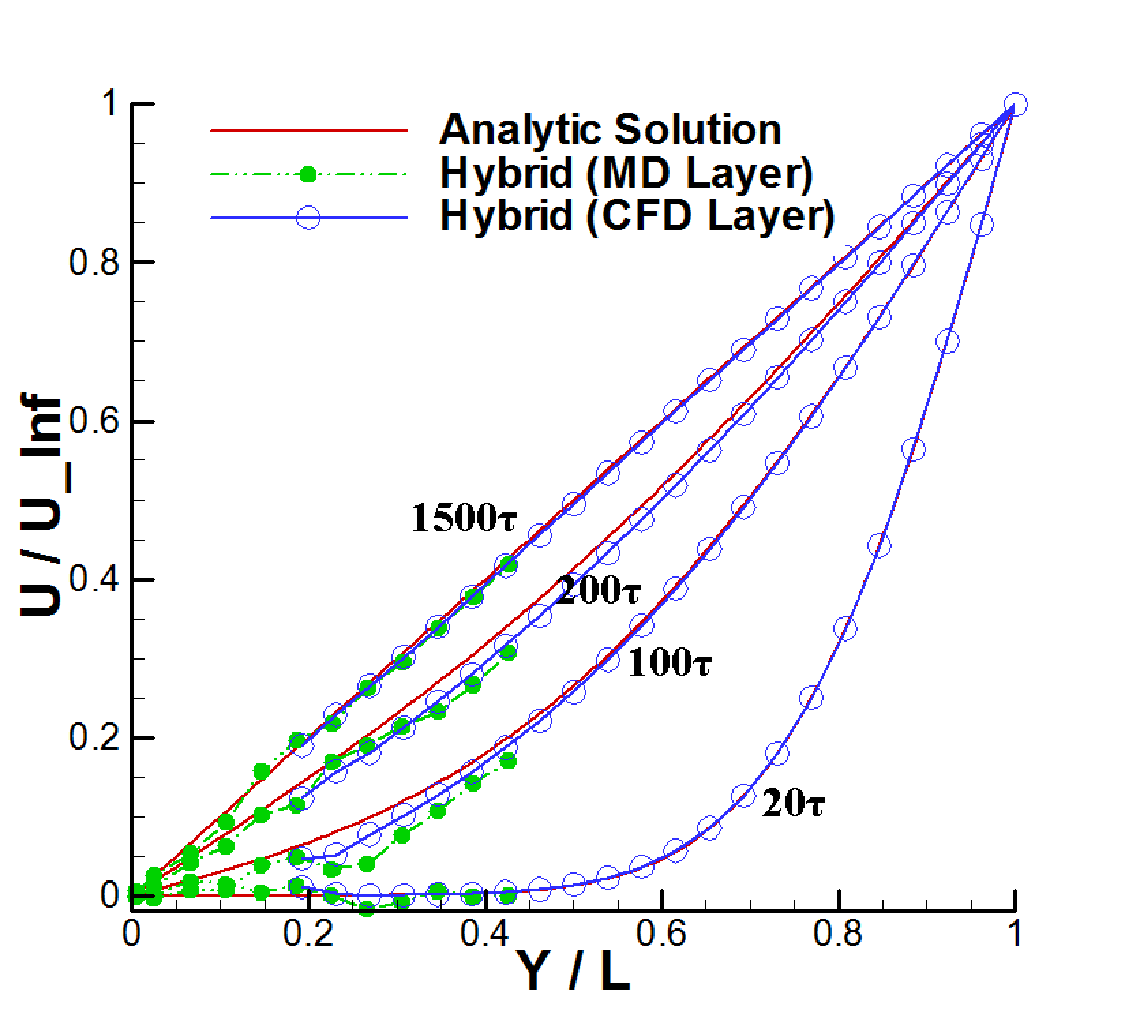
\includegraphics[width=0.6\linewidth]{Flat_Plate_Sol2.pdf}}
\vskip-0.2cm
\caption[]{\small {\bf Time evolution of impulsively started Couette flow velocity profiles with upper plate velocity of  $\sigma/\tau$.} The CFD solution is the instantaneous profile at the time indicated and the MD solution is spatially averaged over a slab of height 2$\sigma$ and temporally averaged over 10$\tau$. (a) Pure CFD solution compared to the MD solution and the analytical solution. (b) Hybrid solution compared to the analytic solution.
%A time-accurate Couette flow profile.} The evolution of velocity field along the vertical direction is presented. CFD solution is the instantaneous profile at specified time and MD solution is spatially averaged over 2 $\sigma$ in height and temporally averaged for 1 sampling durations (=10$\tau$).
%\subref{cfd_md_couette} Pure CFD solution is exactly the same as analytic solution. MD solution shows the same flow pattern as analytic solution, though some fluctuation is observed. This verifies that CFD and MD represents the same flow physics.
%\subref{hybrid_couette} The steady result by a hybrid approach produces the same numerical result as analytic solution, though the slight time-lagging in the hybrid boundary is observed during the evolution.
}
\label{Flat_Plate_Sol}
\end{figure}

However, from the practical standpoint, the velocity imposed as a boundary condition on the moving wall in these simulations is rather unrealistically high, considering the nanometer-level distance between two parallel walls. The good agreement of the MD solutions (both pure and hybrid) with theory is not surprising, considering that the mean velocity in these simulations is sufficiently high with respect to the thermal fluctuation velocity in most of the domain. From basic principles, lower, more realistic upper-wall velocities pose a more significant challenge because of the increase in the required sample size to keep the statistical uncertainty (\emph{aka} noise) low. We have addressed this challenge of solving for a moderate-velocity flow field using the hybrid simulation approach. As discussed in Sec.~\ref{sec:numerical_noise}, the hybrid simulation of low-velocity flow fields is mathematically possible but technically bound by the computing capacity, since the computational domain becomes O($u^2$) times bigger in solving for a O($1/u$) velocity field. In order to mitigate this, we ran O($u^2$) more independent simulations with the same initial and smaller system size. In order to make each simulation independent from the others the initial conditions were randomized for the initiation of the MD calculation by using different random number seeds for the initial particle variables in LAMMPS. 

%However, the flow condition in the above experiment is rather unrealistic, considering the nanometer-level distance between two parallel walls. Thus, we challenge ourselves to solve the moderate-velocity flow field by the hybrid simulation approach. As discussed in Sec.~\ref{sec:numerical_noise}, the hybrid simulation of the low-speed flow field is mathematically possible but technically bound by the computing capacity, since the computational domain becomes $u^2$ times bigger in solving for a $1/u$ velocity field. Instead, we ran $u^2$ independent simulations with the initial system size and different random number seeds in the LAMMPS package.

Fig.~\ref{multiple_couette} presents Couette flow velocity profiles obtained by averaging different numbers of simulations. All configurations and parameters are identical to the validation problem detailed previously except for the upper plate velocity, which is 0.25 $\sigma/\tau$ for the results given in Fig.~\ref{multiple_couette}. Reducing the velocity by 1/4 implies that an average of 16 simulations is required to achieve a solution with a comparable statistical integrity as in the original case of the problem with the higher velocity. The results support this assumption. The reduction of statistical uncertainty (noise) by the multiple simulation or ?eplica?sampling method is clearly visible in Fig.~\ref{multiple_couette_temporal}. The noise is reduced by roughly half when 4 simulations are averaged. The solution from averaging 16 simulations shows further reduction of the noise. 

%Fig.~\ref{multiple_couette} presents the Couette flow profiles at different numbers of samples. All configurations and parameters are identical to the above validation problem except the upper plate velocity of 0.25 $\sigma/\tau$.  Changing the velocity to 1/4 implies that an average of 16 samples is required to achieve an acceptable numerical solution. Our result supports the above supposition. The reduction of statistical noise by the multiple replica sampling is clearly verified in the graph presented in Fig.~\ref{multiple_couette_temporal}. The noise is seen to reduce by roughly half with 4 times more samples. The solution of sampling 16 runs shows about 5$\%$ of the noise compared with the analytic velocity solution.


\begin{figure}
\centering
\subfloat[Sampling of 4 Replicas]{\label{couette_slow_4}
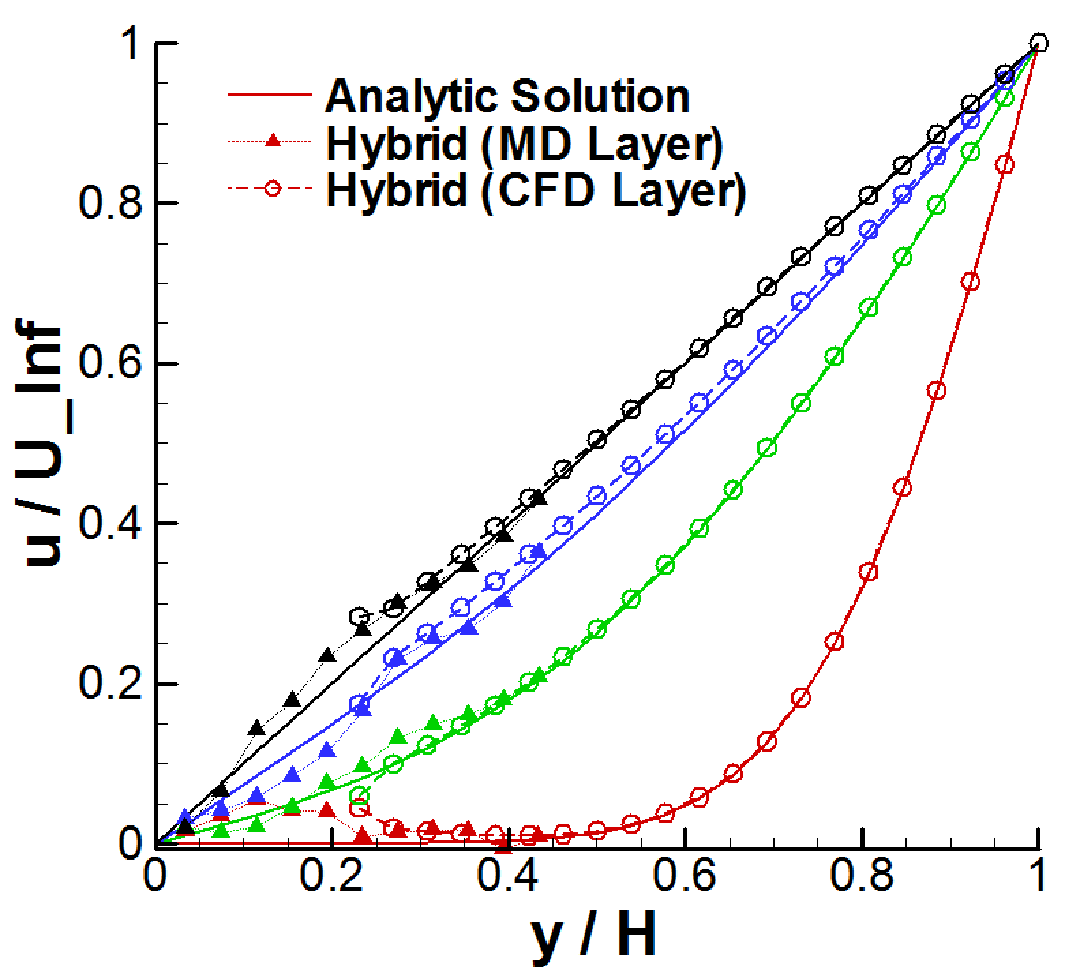
\includegraphics[width=0.6\linewidth]{Couette_025_Samp4.pdf}}
\hskip 1cm
\subfloat[Sampling of 16 Replicas]{\label{couette_slow_16}
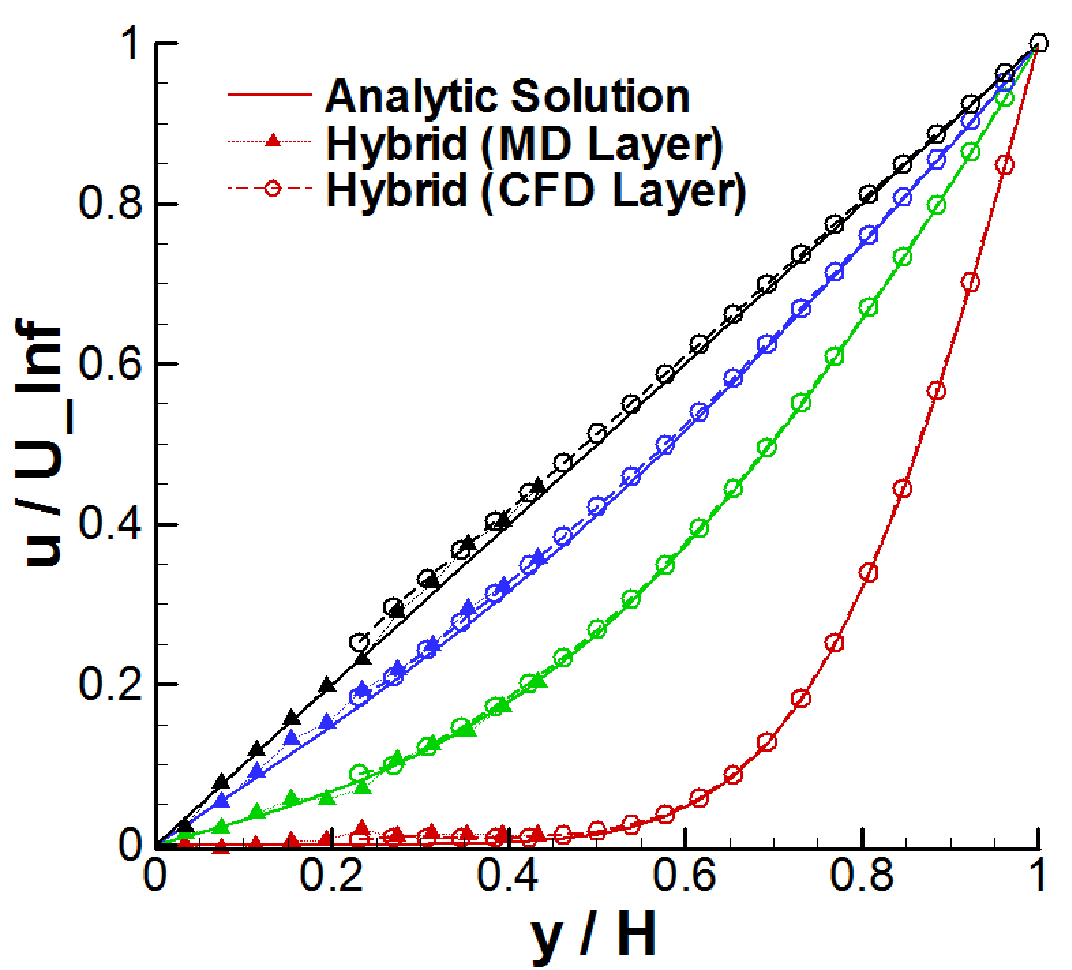
\includegraphics[width=0.6\linewidth]{Couette_025_Samp16.pdf}}
\vskip-0.2cm
\caption[]{\small {\bf Time evolutions of impulsively started Couette flow velocity profiles with upper plate velocity of 0.25$\sigma/\tau$}. 
Illustrating the effect of the number of averaged simulation replicas. Red: t=20$\tau$; Green: t=100$\tau$; Blue: t=200$\tau$; Black: t=1500$\tau$.
%A Couette flow profile with the upper plate velocity of 0.25 $\sigma/\tau$.} The noisy solution when 4 individual simulations are averaged is resolved by sampling 16 independent runs. Red lines denote the solution at 20 $\tau$; Green, blue and black lines are solutions at 100, 200 and 1500 $\tau$, respectively.
}
\label{multiple_couette}
\end{figure}

\begin{figure}
\centering
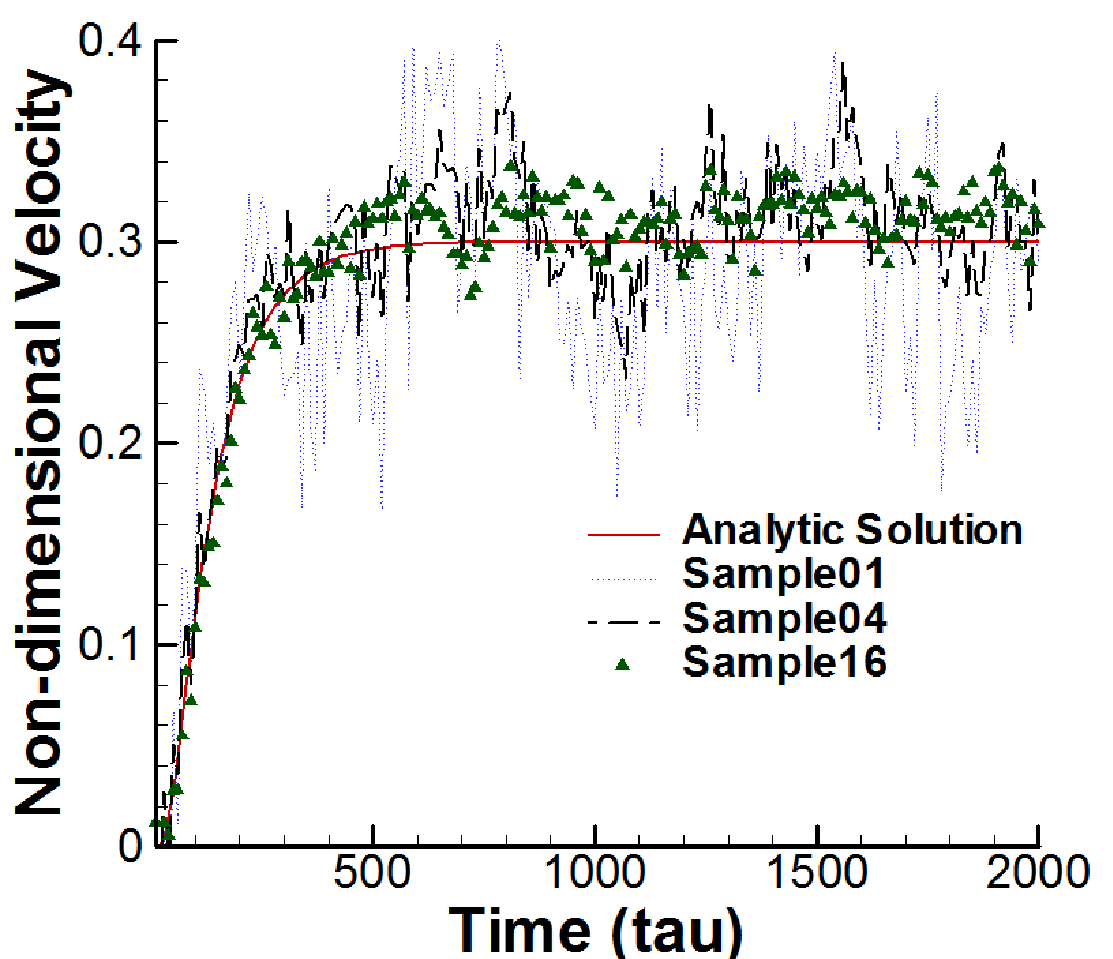
\includegraphics[width=0.6\linewidth]{Couette_025_Temporal_Multiset.pdf}
\vskip-0.2cm
\caption{\small {\bf} Variation of the continuum velocity at the center of the overlapping region for  various cases averaging different numbers of simulation replicas including the analytical solution for comparison. 
%The variation of continuum velocity in the middle of the overlapping region.} Velocity changes at various replica samples are compared with the analytic solution. In case 16 simulations are averaged, the noise is about 5 $\%$ compared to the analytic solution.
}
\label{multiple_couette_temporal}
\end{figure}

In order to verify the equivalence of averaging an increased number of simulation replicas to increasing the size of the domain, the solution obtained by averaging multiple (16) simulation replicas was compared to the solution obtained from a single simulation after increasing the size of the particle system. This was easily achieved by appropriately increasing the size of the domain in the principal direction of motion. Figure~\ref{increase_system}(a) shows the Couette flow velocity profiles from the larger system. Figure~\ref{increase_system}(b) presents a comparison of the temporal variation of the horizontal velocity component, obtained at the center of the overlap region, between the multi-replica and enlarged domain simulations.   Both simulations  produce mutually consistent numerical solutions, which compare well with the analytical solution. The scale of the noise is also roughly the same in both simulations, which verifies that the multiple-replica averaging approach is as effective as that of appropriately enlarging the simulation domain. However, in terms of the total time-to-completion, the multiple-replica averaging approach can be more efficient, because massively large-scaled jobs (in terms of wall-time limit or number of resources requested) have typically lower allocation priority. The labor of multiple job submissions and the post-processing of replicas can also be relieved by the use of the BigJob abstraction.

%We compared the solution by multiple replica sampling with the solution in the increased system domain. Figure~\ref{increase_system} shows the Couette flow profile on a 16 times larger system size in the horizontal direction and the temporal velocity variation by the multiple replica simulation and large domain solution in the middle of the overlapping region. From the result, both ways (multiple replica sampling and increasing system size) produce accurate numerical solutions compared with the analytic solution. The scale of sampling noises are roughly the same between two simulations according to Fig.~\ref{increase_system}, which verifies that the multiple replica sampling apporach is as effective as the increment of the simulation domain. In view of total time-to-complete, multiple replica sampling can be more efficient, because a massively large-scaled job (in view of wall-time limit or number of resources requested) is very hard get allocated. The labor of multiple job submissions and the postprocessing of replicas can be relieved by the use of a BigJob abstraction.


\begin{figure}
\centering
\subfloat[A Single Run at 16 Times Larger Domain]{\label{hybrid_scale16}
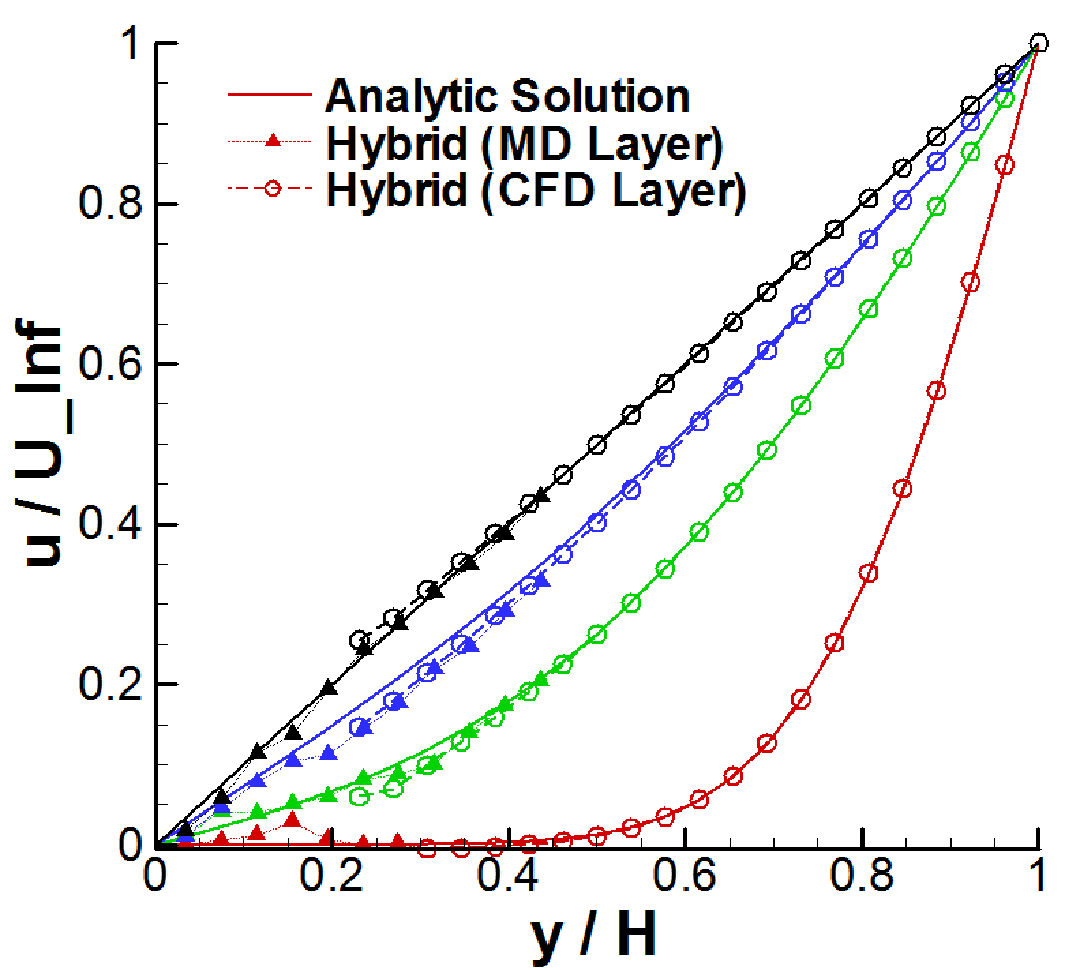
\includegraphics[width=0.6\linewidth]{Couette_025_Scale16.pdf}}
\hskip 1cm
\subfloat[Temporal Variation of Velocity between Replica Sampling and System Increase]{\label{hybrid_history}
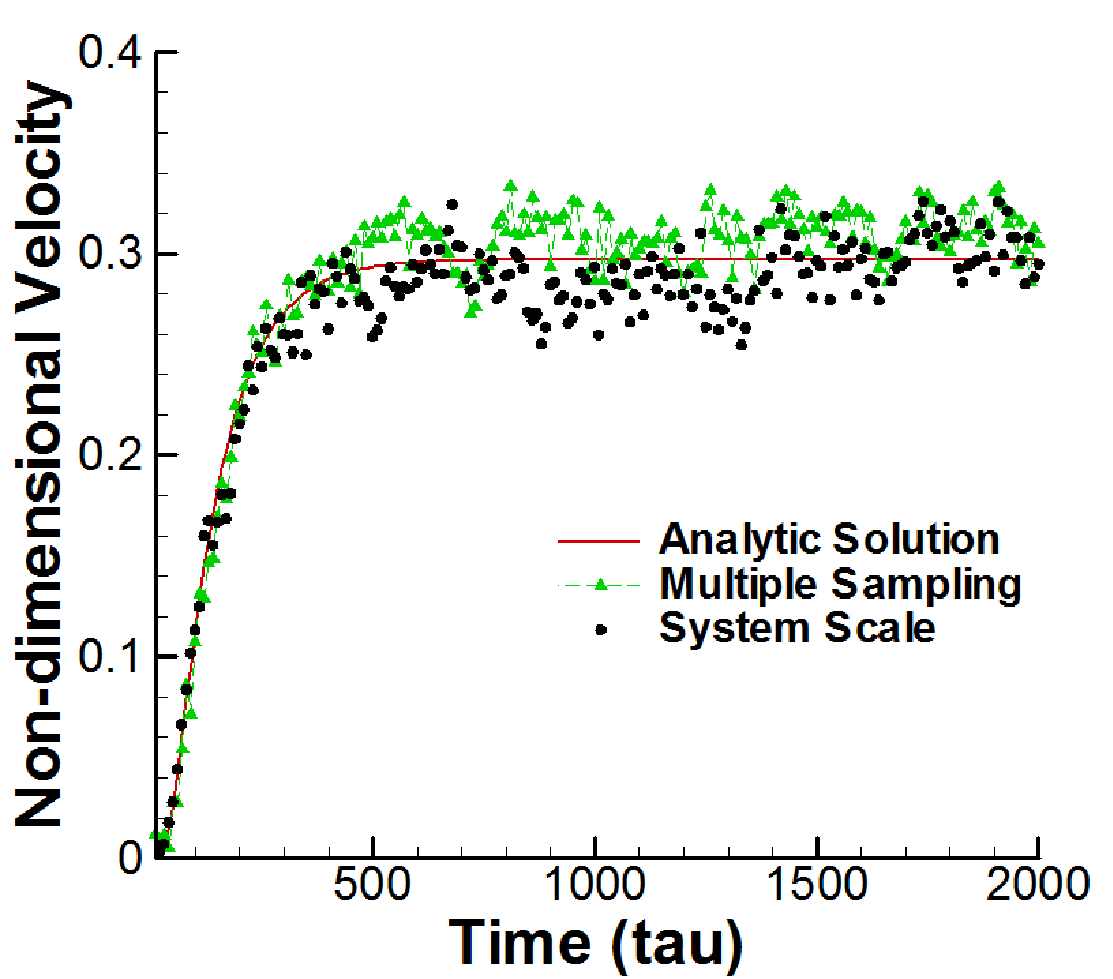
\includegraphics[width=0.6\linewidth]{Couette_025_Temporal_Multiset_VS_Scaleup.pdf}}
\vskip-0.2cm
\caption[]{\small \subref{hybrid_scale16} {\bf A Couette flow profile in increased system size.}  Accurate flow profile can be obtained by increasing the system size 16 times larger when the velocity is reduced to 1/4. Red lines denote the solution at 20 $\tau$; Green, blue and black lines are solutions at 100, 200 and 1500 $\tau$, respectively. 
\subref{hybrid_scale16} {\bf The variation of the velocity in the middle of the overlapping region.} Solutions by multiple replica sampling and increasing the system contain the similar strength of the noise in the solution, which is around 5 $\%$ of analytic velocity profile. This implies that multiple replica sampling approach can replace the increase of system size for solving moderate velocity flow.}
\label{increase_system}
\end{figure}



\subsection{A Physically Unsteady Flow Field: Oscillating Boundary Problem}
\label{sec:accuracy_oscillation}

The accuracy of the designed temporal coupling scheme is verified by solving the unsteady oscillating boundary problem. The flow field converges to a specific profile in a transient flow physics, so the minor disturbance in the middle of flow evolution can possibly be damped out at time of convergence. On the other hand, the local variation at each instance might be incremented/accumulated during the flow evolution, to end up with the completely un-physical solution in case of unsteady flow simulation. Therefore, the accuracy of the temporal coupling scheme becomes more important in the unsteady flow simulation. Suppression of the sampling noise is very important as well, considering the low physical velocity in the hybrid layer. The computational domain and coupling parameters of the current problem are the same as in the above Couette flow simulation. In this case, the upper wall boundary condition changes from the fixed velocity to the oscillatory wall, which is $u_{wall}(t)=({\sigma}/{\tau}){\times}sin(2{\pi}t/T)$. Period $T$ is set to be 200$\tau$.

Figure~\ref{Stokes_Sol} shows the oscillatory velocity profile by pure CFD and hybrid simulations. Figure~\ref{Stokes_Sol}-\subref{vel_stokes} shows that the velocity profiles at each time instance are roughly the same between the pure CFD and hybrid simulations in magnitude. This indicates that the hybrid simulation approach is also applicable to time-varying flow simulations. Meanwhile, the temporal variation of the horizontal velocity in the middle of the hybrid region expresses that the noise in the hybrid solution is not negligible considering the difference between continuum and hybrid velocities. We claim that this noisy solution is caused by the combination of the sampling error and an inaccurate temporal coupling scheme. In order to determine the effect of the temporal coupling scheme, we applied multiple replica sampling over sufficient number of independent experiments and compared solutions from different temporal coupling schemes.


\begin{figure}
\centering
\subfloat[Velocity Profile of an Oscillating Boundary Problem]{\label{vel_stokes}
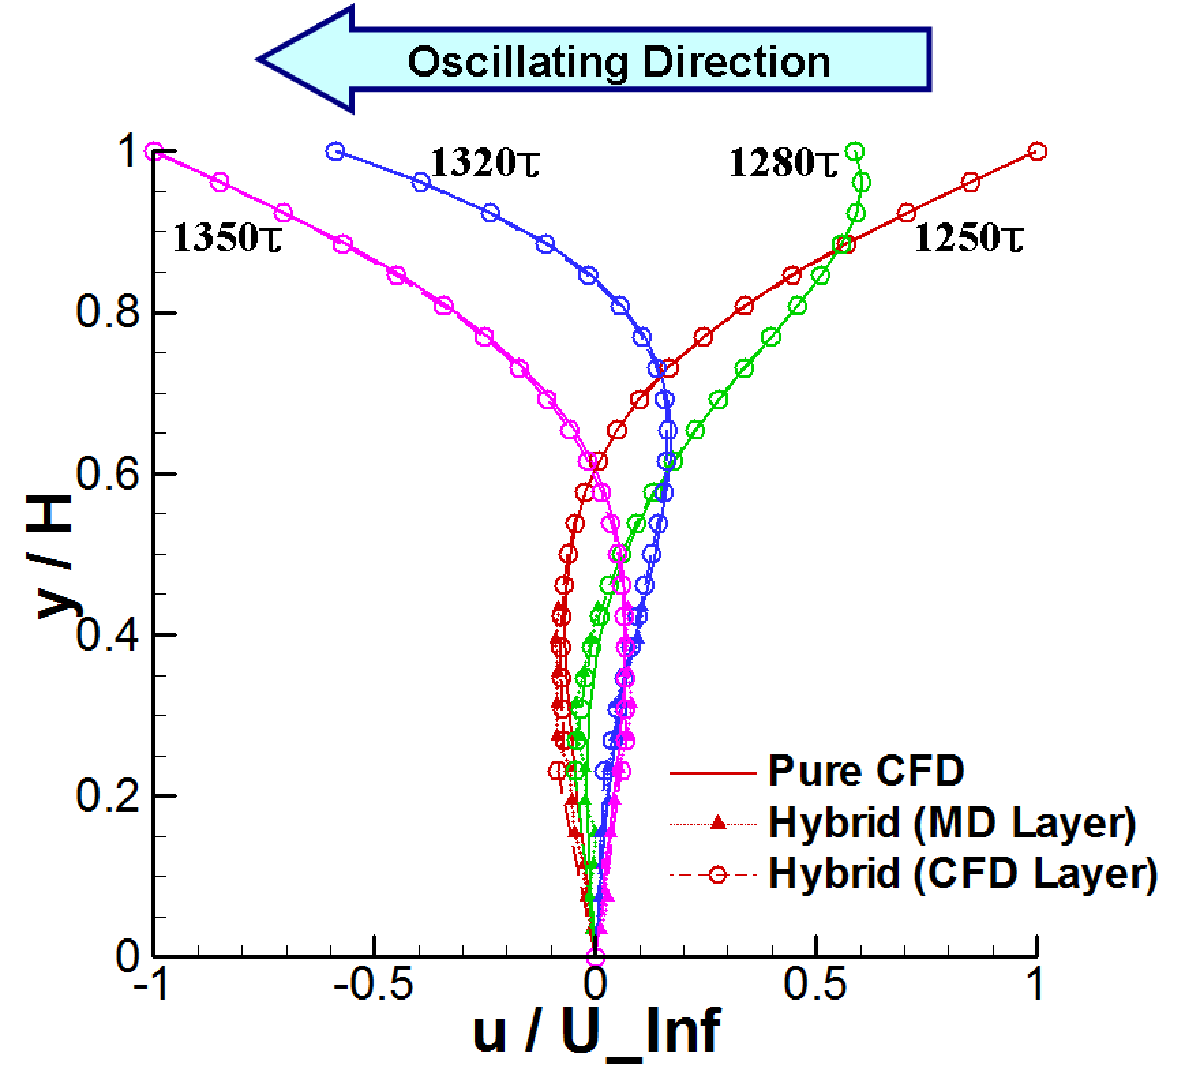
\includegraphics[width=0.6\linewidth]{Stokes_Sol_Profile.pdf}}
\hskip 1cm
\subfloat[Temporal Variation of Velocity in the Middle of Hybrid Region]{\label{vel_stokes_history}
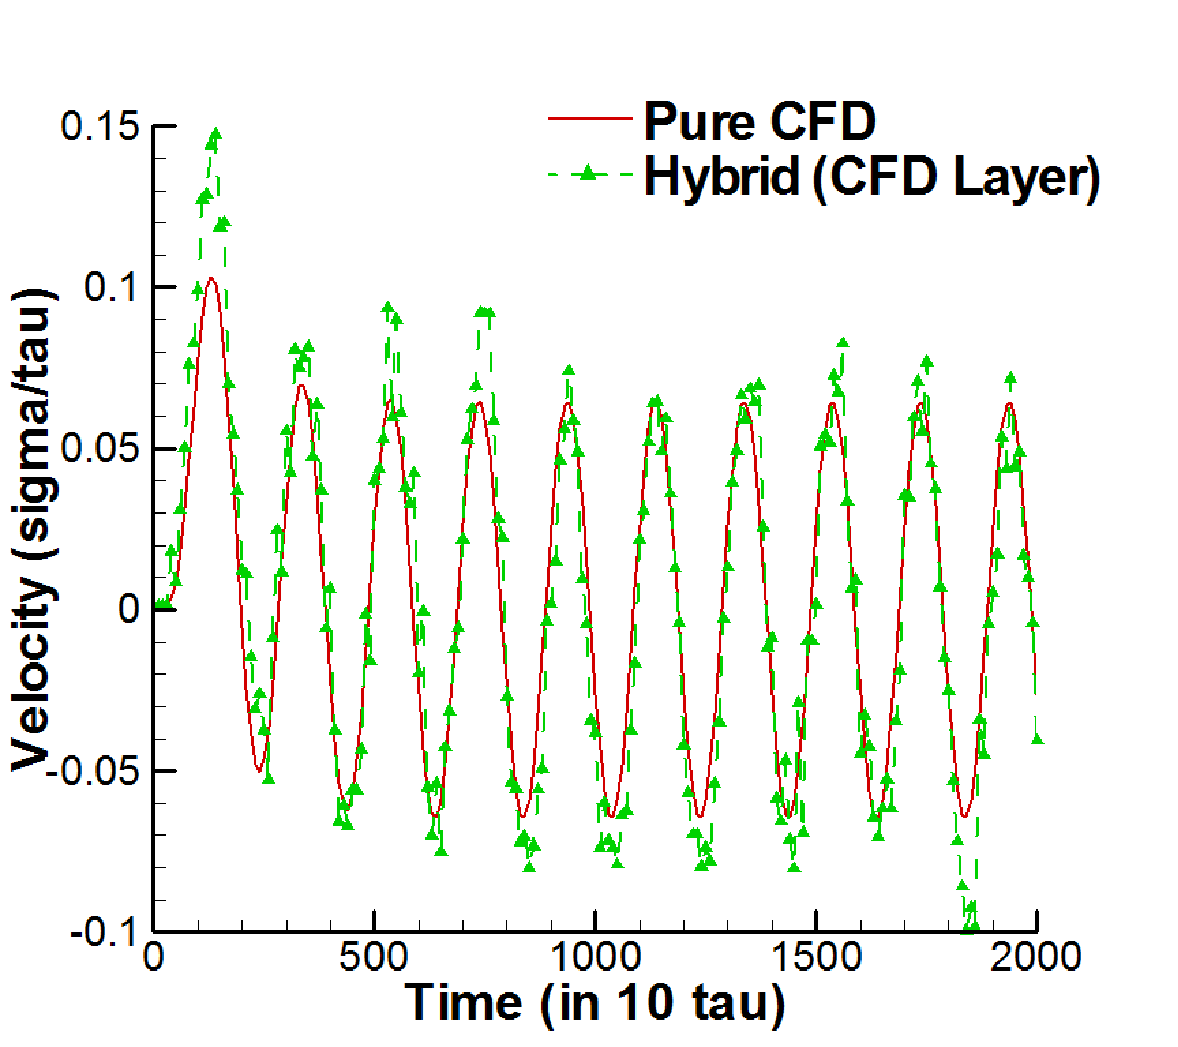
\includegraphics[width=0.6\linewidth]{Stokes_Temporal_Profile.pdf}}
\vskip-0.2cm
\caption[]{\small {\bf A time-accurate flow profile of an oscillating boundary problem.}
\subref{vel_stokes} Difference between hybrid and pure CFD solutions in hybrid region shrinks in the continuum domain. Noise from the MD simulation does not affect the global velocity profile a lot, because the driving force in this simulation is the oscillating velocity from CFD domain.
\subref{vel_stokes_history} History of the velocity field reveals that the hybrid solution contains much noise in this experiment.}
\label{Stokes_Sol}
\end{figure}


We compared velocity history profiles from different temporal coupling schemes. Figure~\ref{Temporal1} indicate a clear difference in the resolution of the overshoot/undershoot phenomena by the prediction-correction approach. A prediction time scale of 2.5 sampling intervals was chosen in the prediction-correction approach to impose the interpolated boundary conditions on both domains. In the conventional model, the maximal error is seen at peak points, which is a natural characteristic of the linear extrapolation in that it fails to predict correct vlaues on a convex/concave graph. This inaccuracy is resolved by a prediction-correction approach with interpolated hybrid boundary conditions. Yet, the time-lagging pattern in the conventional model is still observed in the prediction-correction model, which is expected to be resolved by the adoption of a higher-order interpolation scheme.


\begin{figure}
\centering
\subfloat[Velocity History at Conventional Synchronized Approach]{\label{stokes_org}
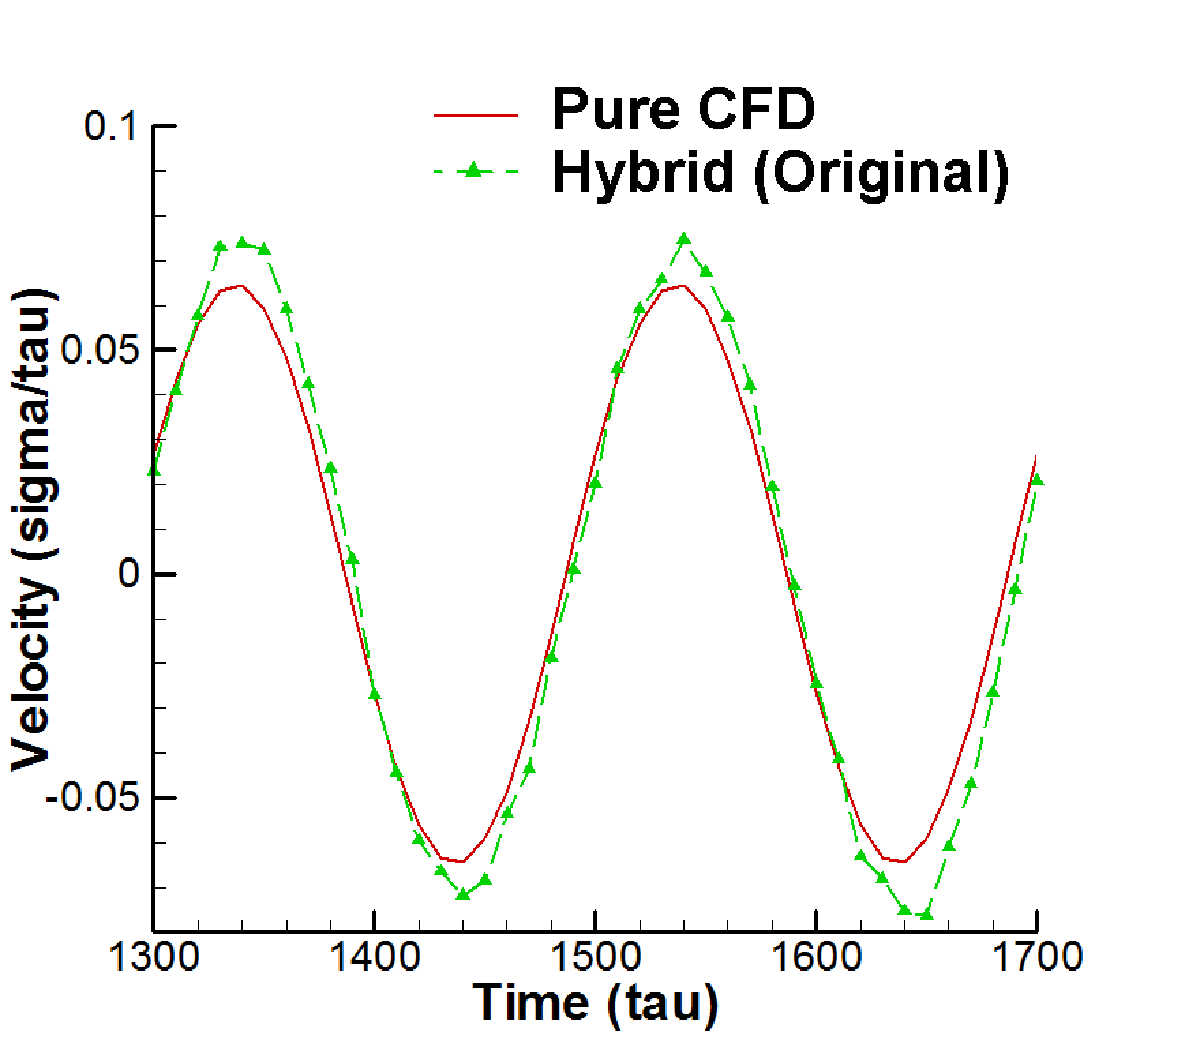
\includegraphics[width=0.6\linewidth]{Stokes_Org_Multi.pdf}}
\hskip 1cm
\subfloat[Velocity History at Prediction-Correction Approach]{\label{stokes_both}
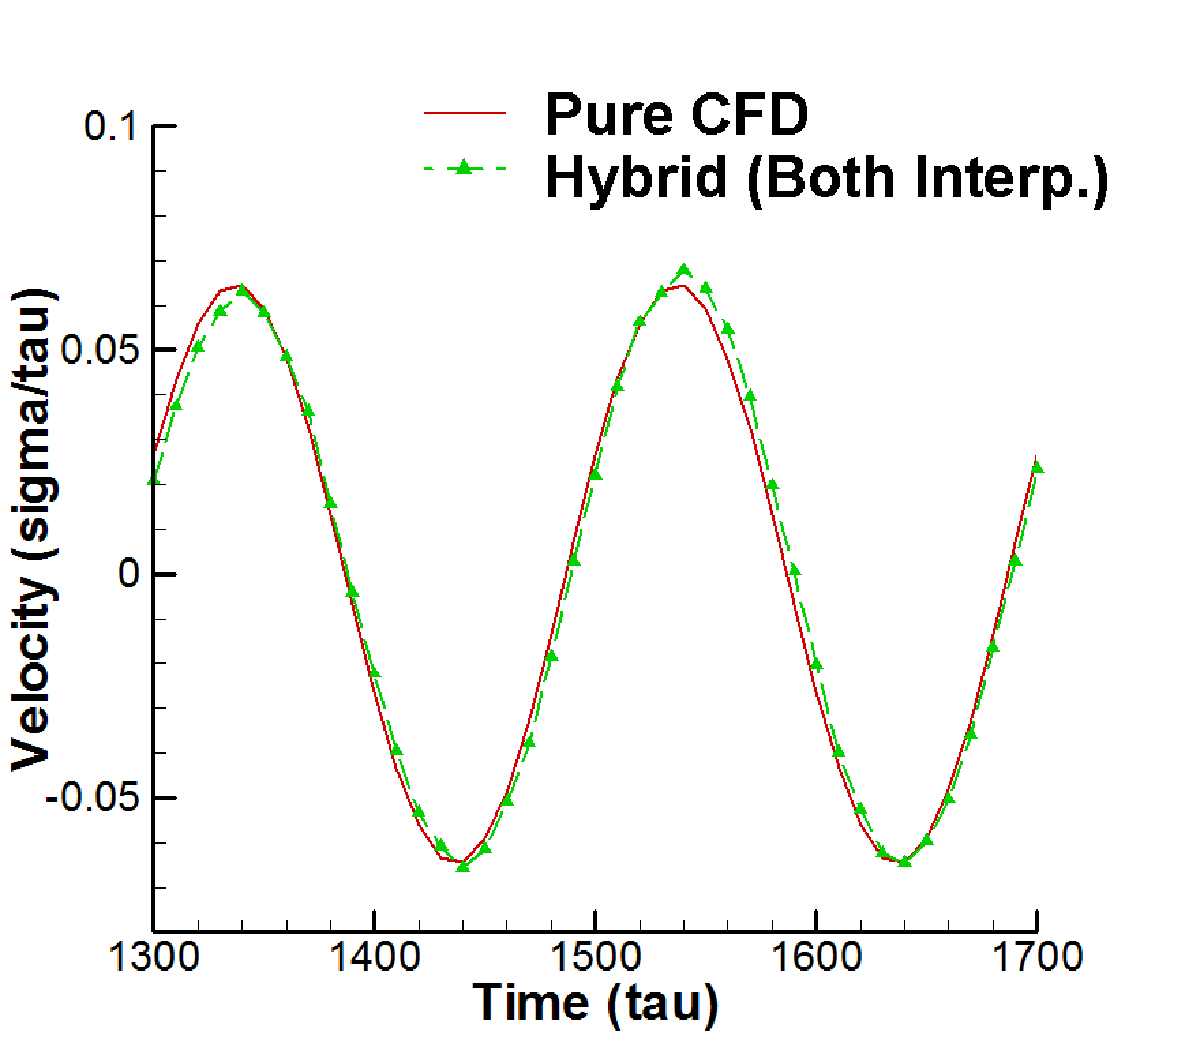
\includegraphics[width=0.6\linewidth]{Stokes_Both_Multi.pdf}}
\vskip-0.2cm
\caption[]{\small {\bf The temporal variation of the velocity in the middle of an overlapping region.}
\subref{stokes_org} With conventional synchronized coupling model, large overshoot/undershoot phenomena are observed on the peak points: the statistical noise around 0.01 $\sigma/\tau$ is nearly 20 $\%$ of the continuum velocity in that location. The time-lagging effect is also captured.
\subref{stokes_both} Overshoot/undershoot phenomena in the conventional approach is almost resolved by applying the prediction-correction approach. The interpolated hybrid boundary conditions are imposed on CFD and MD domains.}
\label{Temporal1}
\end{figure}


The plots shown in Fig.~\ref{Temporal2} quantify the scale of inaccuracy according to the imposition of the hybrid boundary condition. In the conventional model, the velocity difference ranges from -0.017 to 0.015 $\sigma/\tau$. The magnitude of this error reduces as we apply the prediction-correction approach and increase the prediction time scale from 0.5 (corrected extrapolation) to 1.5 (MD interpolation) and 2.5 (both interpolation) sampling intervals. The clear difference between the conventional extrapolation model and corrected extrapolation in the prediction-correction approach demonstrates that the extrapolation from ''previous'' properties can contain far more inaccuracy than extrapolating from the current solution. The similar noise level between corrected extrapolation and MD interpolation express that the accuracy of the hybrid solution is equally affected by the accuracy of each solver. At last, the solution error in the conventional model is roughly reduced by half with the imposition of interpolated boundary conditions on both domains. 


\begin{figure}
\centering
\subfloat[Conventional Synchronized Coupling with Extrapolation]{\label{stokes_org_diff}
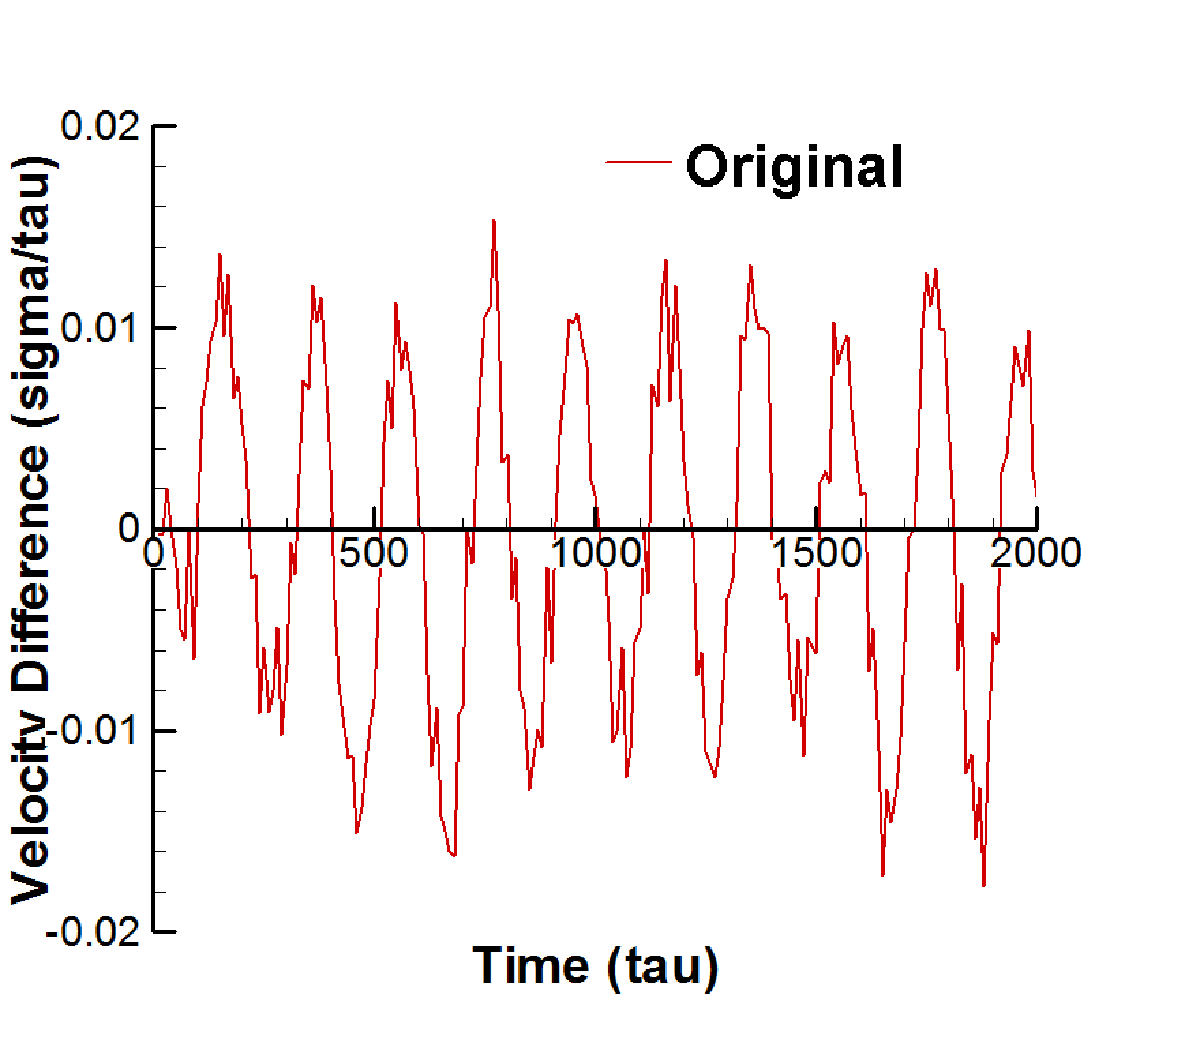
\includegraphics[width=0.4\linewidth]{Stokes_Org_Diff.pdf}}
\hskip 1cm
\subfloat[Prediction-Correction with Extrapolation]{\label{stokes_exp_diff}
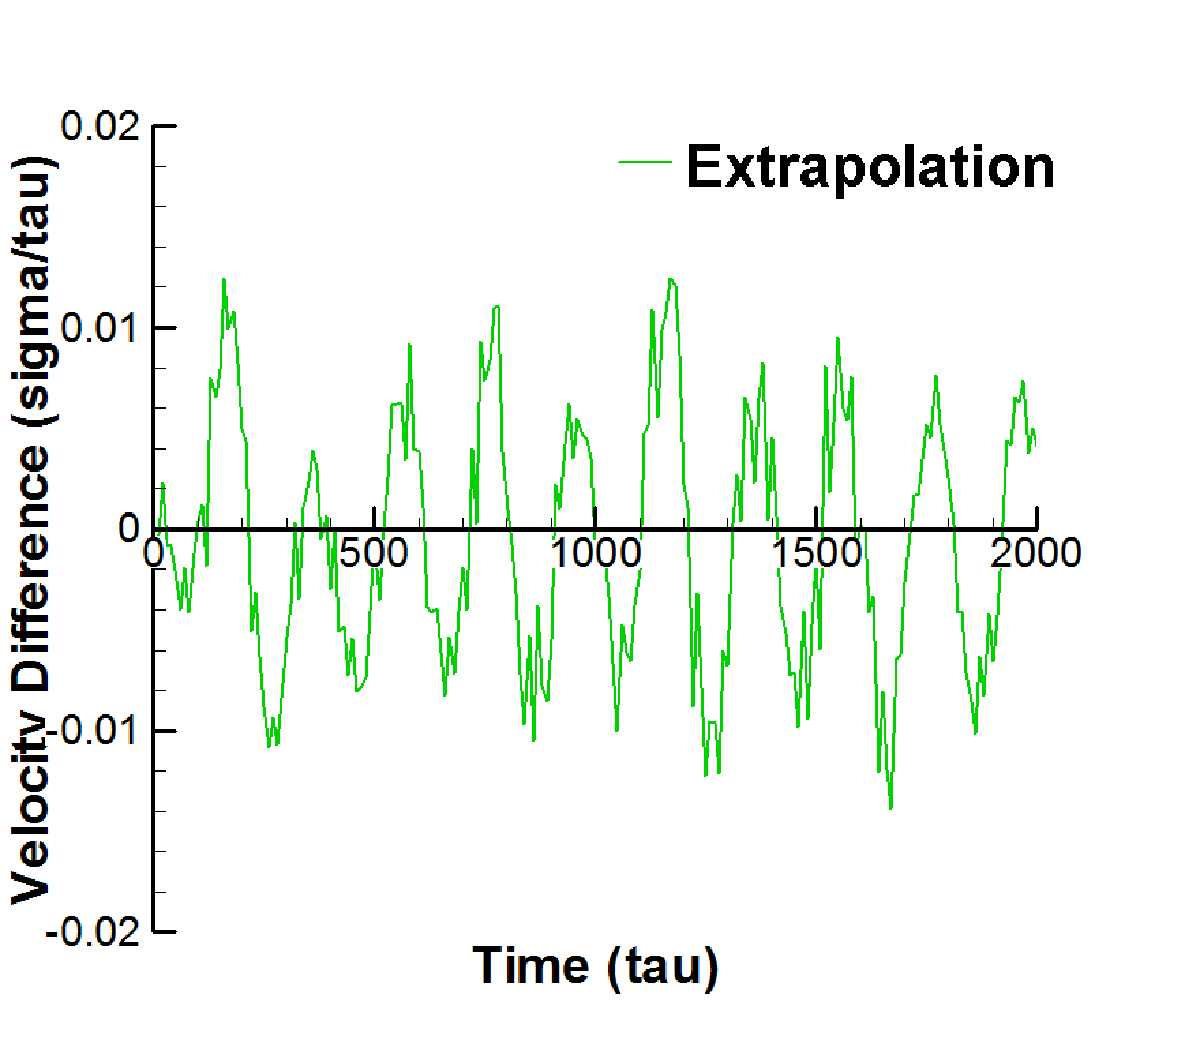
\includegraphics[width=0.4\linewidth]{Stokes_Exp_Diff.pdf}}
\vskip-0.2cm
\subfloat[Prediction-Correction with Interpolation on MD Boundary]{\label{stokes_imp_diff}
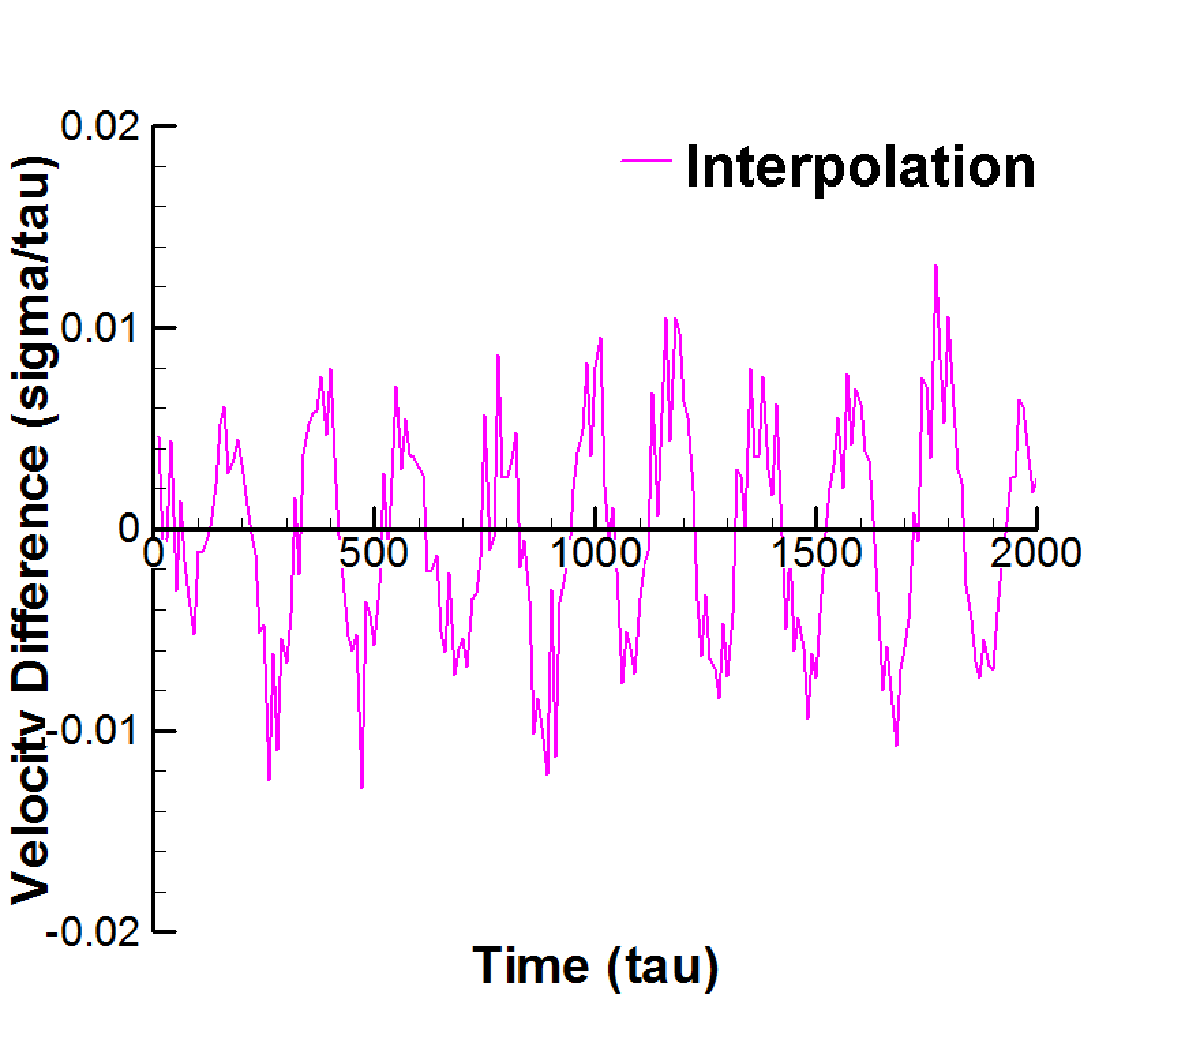
\includegraphics[width=0.4\linewidth]{Stokes_Imp_Diff.pdf}}
\hskip 1cm
\subfloat[Prediction-Correction with Interpolation on Both Domains]{\label{stokes_both_diff}
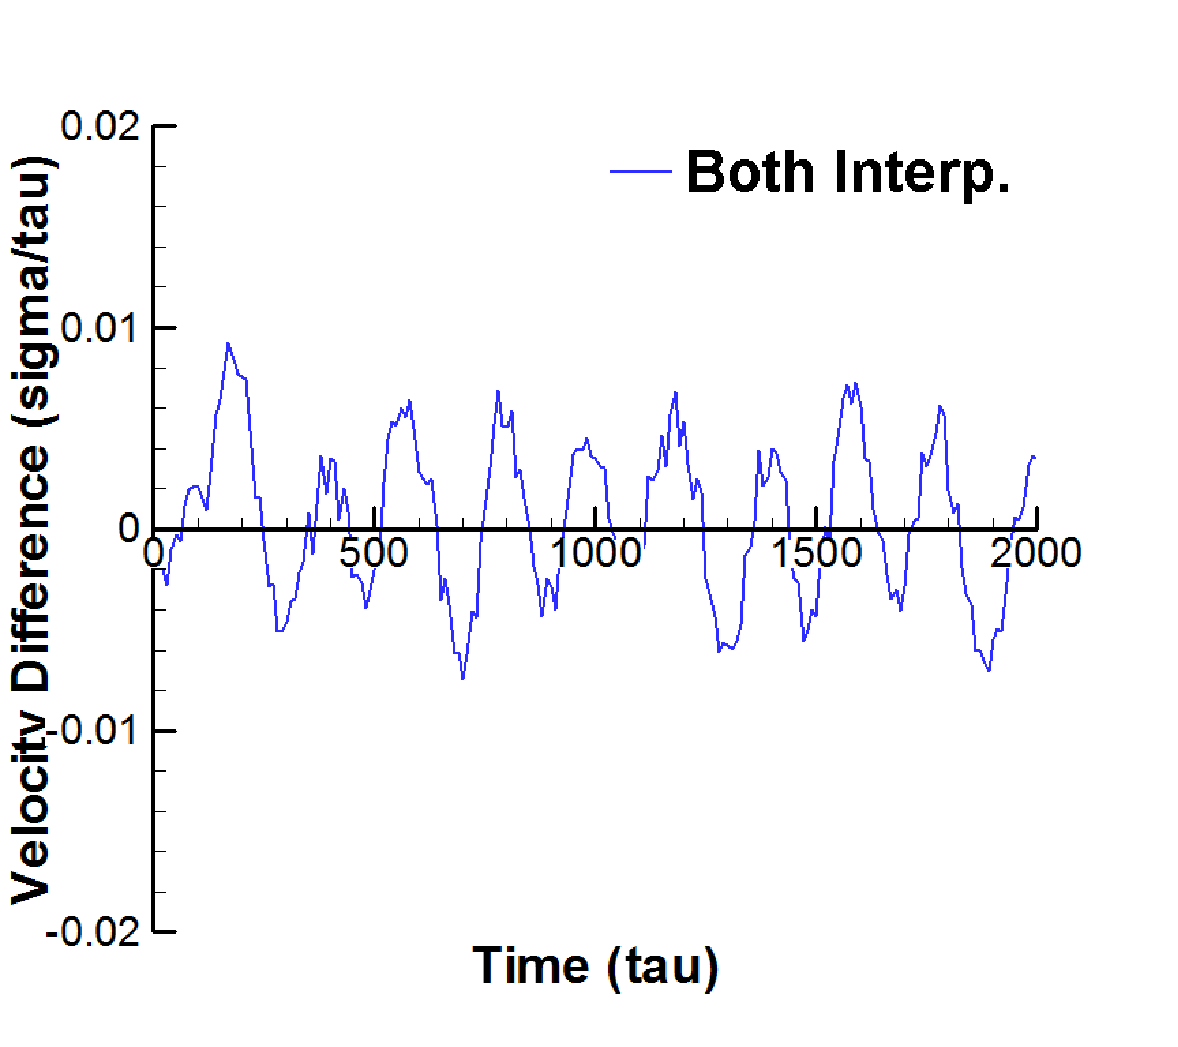
\includegraphics[width=0.4\linewidth]{Stokes_Both_Diff.pdf}}
\caption[]{\small {\bf The reduction of unsteady error by a prediction-correction approach.} Figures show the velocity difference between pure CFD and hybrid solutions in the middle of hybrid layer. Plotted data include the conventional extrapolation model and 3 different types of prediction-correction approaches, which are corrected extrapolation model, interpolated boundary model on MD domain and interpolated boundary condition on both domains. The velocity difference in the conventional model ranges from -0.017 to 0.015. This error reduces to -0.007 and 0.009 at the prediction-correction model.}
\label{Temporal2}
\end{figure}



\section{Performance Analysis of a Multi-physics Simulation Framework}
\label{sec:performance}

The BigJob framework is expected to have a shorter total runtime in a coupled multi-task simulation than conventional (and direct) job submissions. The logical bases are as follows:
\begin{enumerate}
\item Many supercomputing centers adopt a queueing policy of assigning higher priority to bigger jobs, which increases the probability that bigger-sized task are allocated faster than the smaller one(s).
\item Independlently submitted multiple tasks are usually allocated at different physical time. Therefore, the requested wall-time limit should be sufficiently large to cover both maximal waiting time and computation time in case of coupled simulations. On the other hand, co-scheduling of coupled tasks is inherently guaranteed in a packaged job. Therefore the wall-time limit can be determined according to the actual computation time.
\item Load-balancing among multiple tasks can be dynamically achieved dynamically by changing the resource allocation to individual task during the simulation. This change is be possible only when coupled yet distributed tasks are scheduled in the umbrella of a packaged job.
\end{enumerate}

In this section, we present our numerical experiments to verify the above reasons.


\subsection{Waiting Time according to the Size and Wall-time Limit of an Individual Job}
\label{sec:performance_preliminary}

Although many factors affect the waiting times, arguably the most important are existing job requests by the resource at the instant of submission, requested wall-time limits, and the number of processors requested. Two other factors are the backfilling capability (which allows the running of a small job between higher priority jobs with larger and longer resource requests) and the changes in the priority of the test job when a particular higher priority job joins the queue. Among these factors, the number of requested resources and wall-time limits can be handled by users and systematically accounted for.

We designed experiments to determine if running larger and/or longer simulations affects the actual waiting time in the queue. We submitted jobs of different sizes and different wall-time limits at the same time. Each time we submitted a job, we gathered the actual waiting time in the queue. We performed our experiments on a sufficiently large and crowded system of around 65000 cores. We argue that the use of this large and crowded system increases the credibility of our experiments: it reduces the possibility of self-interference between our job submissions (i.e., our requests are allocated in a succeeding pattern). Considering the internal queuing policy of supercomputing centers, such as credential, fair share, resource and service priority, each user account has a restricted number of concurrent job submission, and the allocation history affects the priority of the next submitted job. Thus, we submitted different wall-time limit jobs from different user accounts in the same group allocation, and we allowed enough idling time between individual experiments to recover the priority of each account to the initial level. Results from 10 independent experiments were averaged for measurement.

Table~\ref{table:WaitTime} demonstrates the queue waiting time according to the size and wall-time limit of the job. Regarding the influence of job sizes on waiting time, jobs with larger core counts have typically lower wait times, with the exception at 128 cores which is presumably affected by the backfilling capability. Waiting time with 1000+ cores shows a stiff decrease particularly because it is granted higher priority in this queuing policy. The same applies to the increase in waiting time to the wall-time limit of 48, which is administrated by a different queue. The effect of the wall-time limit on waiting time is not clear in our experiment, in the case where they are in the same queue (6- and 24-hour jobs). Collectively, submitting a BigJob for the coupled simulation instead of individually submitting multiple smaller tasks \textit{at least} provides the comparable waiting times in the queue even when small jobs are "ideally" allocated (i.e., all jobs are allocated at the same time).


\begin{table}
  \caption{\small {\bf The effect of job conditions on waiting times.} The tables show the queue waiting times depending on the number of cores and requested wall-time limits. Measurements are made on Ranger system, which is a TeraGrid resource located at Texas Advanced Computing Center. Analyzing the actual waiting time as a function of the number of cores at different wall-time limits, it can be said that better more often than not, the waiting time decrease as the requested number of cores increases. The relationship between the waiting time and wall-time limit is harder to quantify. However, obtained numbers provide a good case study for showing the variance of actual queue waiting times. 
10 independent experiments are sampled and expressed in seconds as "mean$\pm$SD".}
  \label{table:WaitTime}
  \centering\footnotesize
  \begin{tabular}{c || c c c}
 \multicolumn{4}{c}{\phantom{\tiny 100}}\\
\hline
 \multirow{2}{0.15\textwidth}{Number of Processors} &
 \multicolumn{3}{c}{Requested Wall-time on Ranger} \\
\cline{2-4}
& 6 Hrs & 24 Hrs & 48 Hrs\\
\hline			
128  &  24287.14\scriptsize{$\pm$15724.91}  &  25941.71\scriptsize{$\pm$13878.78}  &  44012.14\scriptsize{$\pm$44537.75} \\
256  &  27606.57\scriptsize{$\pm$19207.95}  &  26878.86\scriptsize{$\pm$15108.29}  &  67876.29\scriptsize{$\pm$70713.95} \\
512  &  27930.43\scriptsize{$\pm$18496.98}  &  24361.43\scriptsize{$\pm$14849.23}  &  32097.14\scriptsize{$\pm$27617.86} \\
1024  &  13514.57\scriptsize{$\pm$11373.68}  &  16372.43\scriptsize{$\pm$10857.48}  &  22134.71\scriptsize{$\pm$11089.26} \\
\hline
\end{tabular}
\vspace{-1em}
\end{table}



\subsection{Waiting Time for a Coupled Simulation}
\label{sec:performance_waiting}

Regarding the scenario maps in Fig.~\ref{Fig:BigJob_Structure}, the result in Sec.~\ref{sec:preliminary} provides the waiting time between a BigJob and a first-allocated conventional task. We expect more performance gain by eliminating the inactive idling time (i.e., the difference between the waiting times of the two jobs) with the BigJob application. 

Table\ref{table:BJwaiting}  presents the waiting time of a BigJob sized 2X and two conventional job submissions sized X each. We experimented with two different wall-time limits (6 and 24 hours) and two different processor requests (256 and 512 cores in total). A BigJob submission shows faster allocation, except a small number of processors are requested for a long time, although the waiting time for the first-to-start job was smaller in the conventional job submission mode (S0) than in the BigJob (S1) application. Interestingly, the inactive mode in conventional job submissions was observed to increase substantially as the wall-time limit increased: users get to waste more allocation time as they increase the wall-time limit. From the result, bigger and longer jobs tend to start faster (comparing individual experiments), but it is difficult to affirm this tendency as a general phenomenon because individual experiments were performed at different times.


\begin{table}
  \caption{\small {\bf Waiting and inactive time for conventional job submissions, and a single BigJob submission.} Average of 10 independent runs are presented in seconds. In the first two cases, conventional job is submitted to use 2$\times$128 cores and a BigJob requests 256 cores: latter two cases use 2$\times$256 and 512 cores, respectively. Conventional job submission mode showed faster time-to-start (i.e., waiting time of the first job + inactive mode) with 24 hr - 256 core request, and a BigJob is allocated faster in all other cases.}
\label{table:BJwaiting}
\centering\footnotesize
 \begin{tabular}{c | c | c | c }
 \multicolumn{4}{c}{\phantom{\tiny 100}}\\
\hline
Number of Cores & Wall-time & Scenario & Time-to-start\\
\hline
\hline
\multirow{4}{0.1\textwidth}{256} & \multirow{2}{0.1\textwidth}{6 Hrs} & S0 & 20237.9 + 1045.3\\
\cline{3-4}
&  & S1 & 19720.3\\
\cline{2-4}
& \multirow{2}{0.1\textwidth}{24 Hrs} & S0 & 5035.8 + 9933.3\\
\cline{3-4}
&  & S1 & 16165.0\\
\hline
 \multirow{4}{0.1\textwidth}{512}& \multirow{2}{0.1\textwidth}{6 Hrs} & S0 & 15515.7 + 446.1\\
\cline{3-4}
&  & S1 & 15825.4\\
\cline{2-4}
& \multirow{2}{0.1\textwidth}{24 Hrs} & S0 & 4182.6 + 11096.3\\
\cline{3-4}
&  & S1 & 13627.9\\
\hline
\end{tabular}
\vspace{-1em}
\end{table}



\subsection{Performance Gain through Load Balancing}
\label{sec:performance_LoadBalancing}

A BigJob framework in itself does not provide any performance gain during the simulation: a load balancer (LB) in a BigJob framework provides better parallel performance by redistributing processors to individual tasks within the context of the packaged job. LB measures the performance of individual tasks during a temporary stop and evolves application codes with a changed number of processors. Thus, each code is scheduled to stop and restart several times for the complete simulation, necessitating the capability of a application-level check-pointing and generic domain partitioning routine in application codes (both of which are incorporated capacities in most legacy codes).

The benefit of a LB in a BigJob framework is that it can be applied to any type of coupled applications. On the other hand, it is not highly recommended for the current application for two reasons: 1) in a hybrid CFD-MD simulation, MD usually requires far more computing power than most resources that are dedicated to molecular dynamic simulation; 2) computational cost for the current application in Sec.~\ref{sec:accuracy} is so small that it is not necessary to apply the load-balancing capability. These reasons led us to increase the computational cost of each simulation for evaluating the LB in a BigJob framework. In this experiment, the CFD domain size is increased by 500 times and the MD domain is increased by 20 times. Both CFD and MD codes are scheduled to have 10 simulation loops: start with the same number of processors and experience nine stop-and-restarts with changed resource allocation according to the result of the LB.

The runtimes of the coupled simulation with a single BigJob are shown in Table~\ref{table:oneBJ_Test}. In all scenarios, the same numbers of processors were initially assigned to CFD and MD simulations. Processors distribution in S1\lb changed during the simulation according to the result of the LB function. For both simulations, the time difference between S0 and S1 is within 1\%, which explains why the possible overhead of a BigJob due to communication with the advert server (for monitoring the status of sub-jobs) is negligible. In cases of load-balanced BigJob simulations, there is a significant reduction in the runtime (23.1\%) compared with the default BigJob application when 256 processors are used. For a larger problem set, the performance gain through the application of a LB is relatively small (7.0\%), the reason for which is discussed below.


\begin{table}
  \caption{\small {\bf Simulation runtimes for S0 (conventional job submissions), S1 (default BigJob) and S1\lb (a BigJob with load-balancing).} 256 and 512 cores are used for the coupled simulation. For both cases, S0 and S1 show nearly identical computational cost because the same resource distribution is applied for the coupled simulation. With the load-balancing capability enabled, S1\lb shows about 23.5\% and 6.1\% runtime save compared to S0 when 256 and 512 cores are used. All measured times are in seconds and 5 distinct experiments are averaged.}
\label{table:oneBJ_Test}
\centering\footnotesize
 \begin{tabular}{c | c | c | c }
 \multicolumn{4}{c}{\phantom{\tiny 100}}\\
\hline
\multirow{2}{0.15\textwidth}{Number of Cores} & \multicolumn{3}{c}{Scenario} \\
\cline{2-4} 
& \multirow{1}{0.15\textwidth}{S0} & 
\multirow{1}{0.15\textwidth}{S1} & \multirow{1}{0.15\textwidth}{S1\lb} \\
\hline
\hline
256 & 12306.0 & 12248.7 & 9413.7 \\
512 & 7834.2 & 7910.6 & 7357.6 \\ 
\hline
\end{tabular}
\vspace{-1em}
\end{table}


The validity of a LB can be discussed in terms of the change of processor distribution between sub-jobs throughout the simulation. For the result of the 256 cores (=16 nodes) simulation in Fig.~\ref{Fig:LBSmall}, both CFD and MD subtasks were assigned with 8 nodes initially. From the next simulation loops, the processor distribution converged to 3 to 13 nodes between CFD and MD, respectively. This ratio was maintained throughout the simulation. CFD and MD computation times changed from 260 to 1235 seconds at the initial loop to 705 to 850 seconds after load balancing. Simulation runtimes were measured to be about 35 seconds longer than the slower simulation (MD simulation) per each simulation loop, which is the overhead by the initialization , I/O (input/output) and communication between coupled applications.


\begin{figure}
\centering
\subfloat[Resource Allocation during the Load Balancing Loops]{\label{256_node}
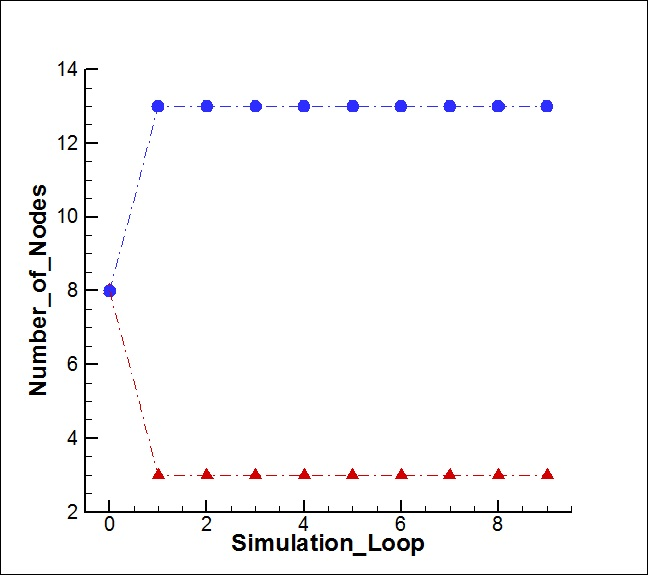
\includegraphics[width=0.4\linewidth]{256_Node.jpg}}
\hskip 1cm
\subfloat[Simulation Time during the Load Balancing Loops]{\label{256_time}
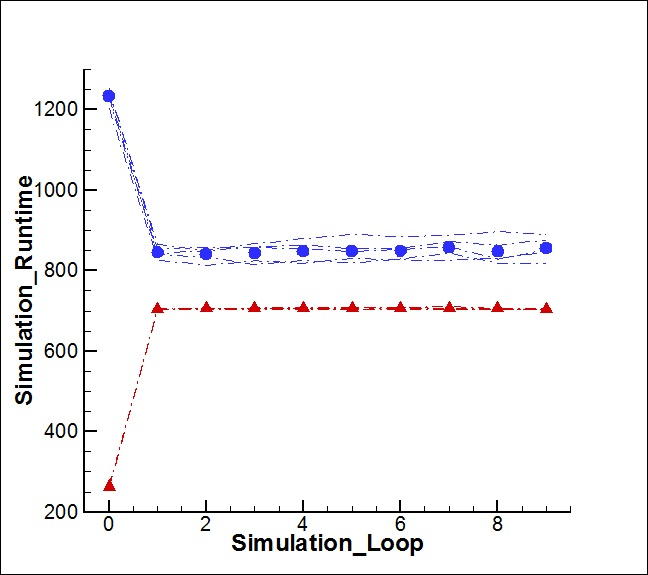
\includegraphics[width=0.4\linewidth]{256_Time.jpg}}
\vskip-0.2cm
\caption[]{\small {\bf Change of resource distribution and computation time between CFD and MD sub-jobs using 256 cores (=16 nodes).} A LB detects the distribution of 3 -- 13 nodes to CFD and MD sub-jobs as the optimal solution. In view of simulation runtime, 1270 seconds for the initial simulation loop reduces to 885 seconds after load-balancing is achieved. Note that each node (which contains 16 cores in the current system) is dedicated to a single application. Triangle and circle symbols denote averaged values from CFD and MD sub-jobs. Dashed lines are solutions from the individual experiment.
}
\label{Fig:LBSmall}
\end{figure}


The result for the case of computation time evolution in 512 cores (=32 nodes) is presented in Fig.~\ref{Fig:LBLarge}. Compared with the above experiment, which uses smaller cores, the load-balancing solution showed a noisier pattern. In detail, an LB failed to find the optimal solution at the first simulation loop, and the node allocation after load balancing fluctuated between 3 -- 29 and 4 -- 28 nodes in each application, which was caused by two reasons. First, the individual code has poor scalability. The initial simulation time for CFD and MD applications measured around 230 and 780 seconds, and the LB proposed a node distribution from 16 -- 16 to 8 -- 24. However, the computation time at the next simulation loop was measured to be 275 and 680 seconds, respectively. Therefore, the LB has to search for the optimal solution one more time. Load balancing functions that are incorporated in schedulers cannot avoid this iterative searching, since they have to manage black-box applications without getting any information to estimate the problem size. Another reason for the fluctuation is the momentary overhead in the computing system. In our experiment, when 28 nodes are used, MD simulation times vary from 610 seconds to 880 seconds, depending on the magnitude of the internal overhead. This variation indicates the necessity of an LB as a self-correcting tool in response to the instability of the system.


\begin{figure}
\centering
\subfloat[Resource Allocation during the Load Balancing Loops]{\label{512_node}
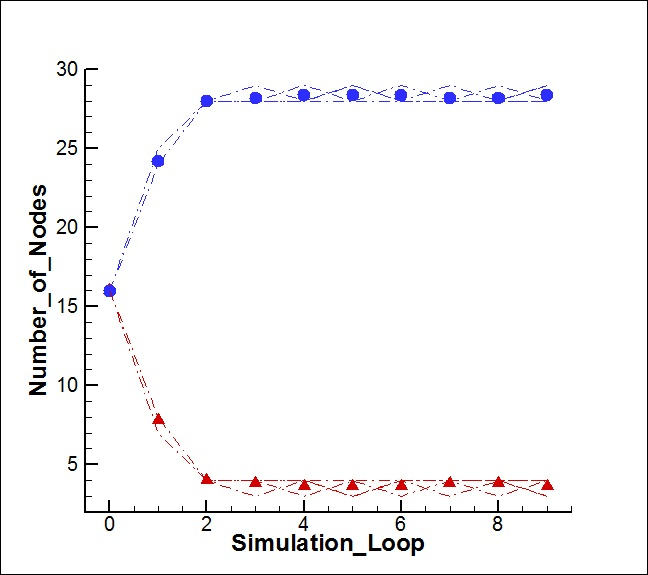
\includegraphics[width=0.4\linewidth]{512_Node.jpg}}
\hskip 1cm
\subfloat[Simulation Time during the Load Balancing Loops]{\label{512_time}
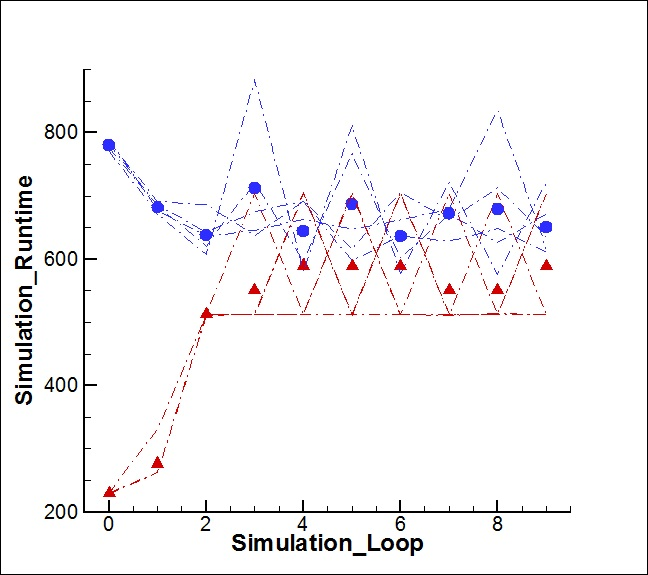
\includegraphics[width=0.4\linewidth]{512_Time.jpg}}
\vskip-0.2cm
\caption[]{\small {\bf Change of resource distribution between CFD and MD sub-jobs and resultant computation time using 512 cores (=32 nodes).} A LB solution fluctuates between 3 -- 29 and 4 -- 28 nodes assigned to CFD and MD sub-jobs, because of temporary internal overhead of a system. Initial simulation runtime around 815 seconds is reduced to be 725 seconds after the load-balancing is achieved, because of the poor scalability of application codes for this problem set. The same caption is used as in Fig.~\ref{Fig:LBSmall}.
}
\label{Fig:LBLarge}
\end{figure}


Two things remained for open discussion: 1) how to effectively measure the actual simulation time of individual task, and 2) how to determine the number of simulation loops. We put time checking routines between the inter-domain communication routine and accumulated the time for running the iteration loop of each code. Based on our knowledge, there is no way to systemically gather the individual simulation times except by this manual deployment. Regarding the number of simulation loops, an excessive number of loops increases the I/O-related overhead (storing the check-pointing solution and restarting from that). An insufficient number of loops increases the simulation time at the initial imbalanced configuration and degrades the capability of the LB for adapting to the unpredicted internal overhead.



\section{Discussion}
\label{sec:conclusion}

Accurate and efficient multi-scale flow simulations by a hybrid CFD-MD simulation framework have been presented in this paper. Hybrid schemes and file-based hybrid interfaces are incorporated in highly-reliable in-house CFD code and LAMMPS molecular dynamics package.They are virtually integrated under a single BigJob abstraction.

The transient Couette flow simulation in O(10) m/s velocity field reports the applicabilty of a hybrid simulation methodology to the non-artificial velocity flow simulation. It has been accomplished by the delicate determination of coupling parameters and the multiple replica sampling approach. Multiple replica sampling refines the statistical error of an individual solution which is significant for the low-speed flow simulation. This approach is superior to simulating a single large-scale problem set in terms of effective scheduling under common batch queue systems, thus it eases the hybrid simulation on most high-performance computing systems. Yet, coupling parameters have been rather intuitively determined according to previous studies and the flow physics, because of the impossibility to predict the strength of sampling noise induced by the solid-liquid interaction. Detailed research is necessary to quantify the variation of statistical error according to the geometric configuration and the interaction with solid obstacle.

The application to the oscillating boundary problem presents the time-accurate flow profile without the numerical overshoot/undershoot phenomena. A prediction-correction temporal coupling scheme contributes to eliminating this unphysical behavior by imposing interpolated properties on hybrid boundaries. We emphasize that the prediction-correction scheme capacitates the accurate unsteady flow simulation. On the other hand, the time-lagging effect on conventional temporal schemes has not been fully resolved by the prediction-correction scheme. We expect that this numerical error can be resolved by applying a higher-order interpolation scheme for hybrid boundary conditions.

Along with numerical issues, computational issues for the efficient coupled simulations have been also discussed. We introduced a BigJob abstraction which provides the co-scheduling capability among logically separated sub-tasks. A simple load-balancing function is also incorporated in a BigJob to achieve the load-balancing among those distributed-yet-coupled codes. From numerical experiments, we evaluate that a BigJob is effective in reducing the waiting time on many supercomputers whose queueing policies encourage high capability simulations. Also, the load-balancing function contributes to reducing the simulation runtime by efficiently distributing allocated resources to sub-tasks. We value that our computational experiments illustrates how to efficiently conduct coupled simulations. Our design concept and the BigJob abstraction can be applied to the similar distributed multi-scale simulations.



\section*{Acknowledgements}
This work is part of the Cybertools (http://cybertools .loni.org)
project and primarily funded by NSF/LEQSF (2007-10)-CyberRII-01.
Important funding for SAGA has been provided by the UK EPSRC grant
number GR/D0766171/1 (via OMII-UK) and HPCOPS NSF-OCI 0710874. This
work has also been made possible thanks to computer resources provided
by TeraGrid TRAC TG-MCB090174 and LONI resources.



\bibliographystyle{elsarticle-num}
\bibliography{Bibs/Hybrid,Bibs/saga,Bibs/saga-related}



\end{document}

